\chapter{Dissipation}
\label{chp_diss}


\section{Introduction}

The analysis of open quantum many-body systems plays an important role in fundamental problems of quantum physics, such as quantum information, quantum computing, decoherence and condensed matter physics. The recent progress in the experimental techniques and the realizations of physical devices for quantum computing gives a further motivation to understand the general behavior of these open quantum systems. They involve a wide class of different specific issues as the study of the non-equilibrium steady state (NESS), the effects of a thermal baths, quantum optics, strongly coupled baths, ...ecc. In particular, in this discussion we focus on the effects of a dissipative process arising from the weakly interaction with Markovian baths. These dissipative mechanisms may lead to emergence of a new collective phenomena which can change completely the physical behavior of the system. In the condition of complete positivity and trace preserving of a dynamical time-evolution map, we can describe the matrix density of the open system using the Lindblad master equation. This equation describes a non-unitary time evolution which provides the dissipative behavior of the observables defined on the system. \\ 
We analyze the dynamic evolution close to a quantum phase transition. In fact, the quantum phase transitions, separating different phases of the system, present universal quantum critical behaviors, which are independent of the local details of the system. They describe the properties of the low-energy spectrum of the system and they show a non-analytical behavior of the ground state, when the size $L^d$ of the system goes to $+\infty\,$ (thermodynamic limit). However, the finite-size effects provide a finite size scaling (FSS) framework in which, approaching the transition point, the observables satisfy peculiar FSS laws. These law characterize the quantum transition giving us a possible way to compare the analytical theory with the results obtained by computational method. We can extend this theory also to dynamical process aring from coherent drivings, as the quench of the Hamiltonian parameters. In these situations, we can provide a dynamic FSS which controls all the out-of-equilibrium regime close to the transitions point. The following step is to understand how a dissipative process drives the system localized near the transition point and how it changes the dynamic FSS. The answer is given for systems in the presence of a homogeneous local dissipation at continuous quantum transition (CQT) \cite{NRV-2019-competingdissipativeandcoherent} and first-order quantum transition (FOQT) \cite{di2020dissipative} in which emerges a new dynamic scaling behavior. However, such a dynamic scaling limit requires a particular tuning of the dissipative interactions so that we have a competition between the critical and the dissipative regime. 

Instead, in the case of dissipative boundaries 
\cite{TV-2021-dissipativeboundaries}, two different dynamic regimes emerge: an early-
time regime for times $t \sim L$, where the competition between coherent and incoherent drivings
develops a dynamic finite-size scaling; and a large-
time regime for $t \sim L^3$ whose dynamic scaling describes the late quantum evolution leading to the
$t \to \infty$ stationary states driven by the Liouvillian gap \eqref{Lioulliangap}.

In the following, we extend this analysis of the dissipative defects effects to a localized particle loss, in one-
dimensional non-interacting lattice fermionic gases confined within a region of size $\ell$. We consider
homogeneous systems within hard walls and inhomogeneous systems where the particles are trapped
by space-dependent external potentials, such as harmonic traps.

Then, finishing to study the peculiar properties of local and homogeneous dissipation, we focus on the importance
of the Liouvillian gap to clarify the interplay between these two different type of dissipation. The aim is
to understand if there is a general theory that describe all the discovered properties.

In conclusion, we start to extend all these concepts in case of thermal bath dissipative systems. Here, we 
consider only the case of quench protocols, but it can be a first step for future research works. 




%\rev{HOMOGENEOUS DISSIPATION}
%\rev{DISSIPATIVE BOUNDARIES}
%\rev{HOLE}
%\rev{THE IMPORTANCE OF THE LIOUVILLIAN GAP TO CLARIFY THE INTERPLAY BETWEEN 
%UNIFORM AND LOCAL DISSIPATION CONFIGURATION. }
%\rev{STARTING TO EXTEND ALL THESE CONCEPTS IN THE CASE OF THERMAL BATH 
%DISSIPATIVE SYSTEMS. HERE, STUDIED ONLY THE CASE OF QUENCH PROTOCOL
%BEHAVIOR}

\section{Out-of-equilibrium dynamics arising from a dissipation hole}

\begin{figure}[!b]
    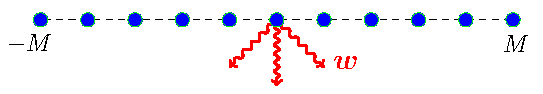
\includegraphics[width=1.0\columnwidth]{imm/sketch.eps}
    \caption{Sketch of a fermionic chain of size $L=2M+1$ subject to a
      localized particle loss at the central site, with strength
      controlled by the dissipation parameter $w$.  }
    \label{fig:sketch}
  \end{figure}
  
  
  As paradigmatic models we consider one-dimensional lattice models of
  non-interacting spinless fermionic gases, within hard-wall and
  harmonic traps, subject to dissipative perturbations that give rise to
  a particle loss localized at one of the sites of the lattice, such as
  the set up sketched in Fig.~\ref{fig:sketch}.  We model the
  dissipative particle-decay mechanism by Lindblad master equations
  governing the time evolution of the density
  matrix~\cite{Lindblad-76,GKS-76,BP-openquantumsystembook,RH-book,dr2021self}.  To
  investigate the effects of the localized particle-loss dissipation, we
  study the quantum dynamics arising from protocols starting from the
  ground state of the fermionic gas, then evolving under the effect of
  the particle-loss dissipation, for example localized at the center of
  the system.  This is analyzed in the large-$\ell$ limit for two
  different initial conditions: fixed number $N_0$ of initial particles
  and fixed ratio $N_0/\ell$, which corresponds to the {\em
    thermodynamic} limit of the initial fermionic gases at equilibrium,
  in both hard walls and harmonic traps.  The quantum evolution of the
  particle number and space-dependent density turns out to develop
  various dynamic scaling regimes, and nontrivial large-time behaviors
  when the dissipative mechanism acts at the center of the system.

  Some issues concerning the behavior of fermionic gases in the presence
  of localized dissipative interactions have been already discussed in
  Refs.~\cite{FCKD-19,LHFHCE-19,KMS-19,WSDK-20,FMKCD-20}, mainly
  for homogeneous systems neglecting boundary effects. Here we extend
  these studies by analyzing the interplay between time, size of the
  system, and number $N_0$ of initial particles. We analyze the various
  large-time and intermediate dynamic regimes, in both homogeneous
  particle systems within hard walls and inhomogeneous particle systems
  in harmonic traps. Substantially different and peculiar behaviors are
  observed in fermionic gases confined by hard walls and harmonic traps.
  
  
  The understanding of the interplay between the time dependence and the
  finite size of the system is essential to interpret results in various
  experimental contexts. For example this issue is fundamental for
  small-size quantum simulators operating on a limited amount of quantum
  objects, in the presence of controlled dissipation. We also mention
  experiments with cold atoms within a trap of finite size, when the
  many-body correlations become eventually sensitive to the trapping
  potential (local density approximations generally fail to describe
  quantum correlations, in particular when they are
  critical~\cite{CTV-13} and/or out-of-equilibrium~\cite{rossini2021coherent}).
  
  
  \subsection{Free lattice fermions  with localized dissipative defects}
  \label{modeldiss}
  
  \subsubsection{The Hamiltonian}
  \label{model}
  
  We consider one-dimensional $N$-particle Fermi gases defined on a
  chain with $L=2M+1$ sites, by the Hamiltonian
  \begin{equation}
    \hat H =
    - \kappa \sum _{x=-M}^{M-1} 
    (\hat c_{x}^\dagger \hat c_{x+1} +  \hat c_{x+1}^\dagger \hat c_{x})\,,
    \label{Hfree}
  \end{equation}
  where $\hat c_x$ is a fermion one-particle operator, and $\hat n_x =
  \hat c_x^\dagger c_x$ is the particle density operator.  We consider
  hard-wall (open) boundary conditions.  The site $x=0$ is the central
  site of the chain.  In the following we set $\hslash=1$ and $\kappa=1$
  without loss of generality.
  
  We also consider fermionic systems where the particles are trapped by
  an external potential, which can be taken into account by adding a
  corresponding term to the Hamiltonian (\ref{Hfree}), such as
  \begin{eqnarray}
    \hat H_t =
    - \sum _x 
    (\hat c_{x}^\dagger \hat c_{x+1} +  \hat c_{x+1}^\dagger \hat c_{x})
  +  \sum_x V(r) \, \hat n_x\,,\label{htrap}
    \end{eqnarray}
  where 
  \begin{eqnarray}
  \hat n_x =
  \hat c_x^\dagger c_x\,,\quad  V(r)= (r/L_t)^p\,, \quad r\equiv |x|\,,
     \label{potential}
  \end{eqnarray}
  $p$ is a positive number, $r$ is the distance from the center $x=0$ of
  the trap, and $L_t$ plays the role of trap size.~\footnote{$L_t$ plays
  the role of trap size~\cite{BDZ-08,RM-04,CV-10-2}, so that the {\em
    thermodynamic} limit is obtained in the large trap-size limit,
  $L_t\to \infty$, keeping the ratio between the particle number $N$ and
  the trap size $L_t$ constant, which can be equivalently obtained by
  adding a chemical-potential term in the Hamiltonian, such as the one
  reported in Eq.~(\ref{chemicalpot}).}  The trapping potential is
  effectively harmonic in most cold-atom experiments~\cite{BDZ-08},
  i.e., $p=2$.  In the limit $p\to\infty$ we recover the model
  (\ref{Hfree}) with hard-wall boundary conditions and $M=\lfloor L_t
  \rfloor$.  The size of systems described by the Hamiltonian $\hat H_t$
  with finite $p$ is supposed to be infinite. However for practical
  purposes it is sufficient to consider models within hard walls with $L
  \gg L_t$. Indeed the large-size convergence is generally fast for
  sufficiently large values of $p$, including $p=2$, due to the fact
  that the average particle density $\langle \hat{n}_x \rangle$ vanishes
  rapidly for $|x|\gg L_t$. The main features of the behavior of fermionic
  gases trapped by a inhomogeneous external power-law potentials have
  been much investigated, see e.g.
  Refs.~\cite{ACV-14,Nigro-17,CV-10,CV-10-2,Pollet-12}.
  
  In systems within both hard-wall and inhomogeneous traps, the particle
  number operator
  \begin{equation}
    \hat{N} = \sum_x \hat n_{x}\,
  \label{partnum}
    \end{equation}
  commutes with both Hamiltonians (\ref{Hfree}) and
  (\ref{htrap}). Therefore the particle number is conserved in both
  cases.  In the following we consider ground states for a number $N_0$
  of particles as starting point of dynamic protocols involving
  dissipative mechanisms.
  
  
  
  \subsubsection{Localized particle-decay dissipation}
  \label{locdiss}
  
  We model the dissipative mechanisms within the Lindblad
  framework~\cite{Lindblad-76,GKS-76}, where the evolution of the matrix
  density $\rho(t)$ of the system is described by he
  equation~\cite{BP-openquantumsystembook,RH-book}
  \eqref{eqlindblad}.
  We recall that the conditions leading to the Lindblad framework are
  typically satisfied in quantum optical
  implementations~\cite{BDS-2015-KeldyshOptical,dr2021self}.  The form of the operator
  ${\mathbb D}[\rho]$ depends on the nature of the dissipation arising
  from the interaction with the bath.  We consider a localized
  particle-decay dissipation acting at the site $z$, modeled by the
  Lindblad operator~\cite{HC-13, KMSFR-17, N-2019-uniquenesslindblad, NRV-2019-competingdissipativeandcoherent, WSDK-20,
    FMKCD-20, dr2021self,rossini2021coherent}
  \begin{eqnarray}
  \mathbb{D}[\rho] = w\,\biggr[
      \hat c_{z}\,\rho\,\hat c_{z}^\dagger - {1\over 2}\left( \rho\,
      \hat c_z^\dagger \hat c_{z} + \hat c_z^\dagger \hat c_{z} \rho \right)
      \biggr] \,, 
  \label{Lindop}
  \end{eqnarray}
  where $w$ is a parameter controlling the strength of the particle-loss
  dissipation.
  Note that reflection symmetry with respect to
    the center of the confined particle system is only preserved when
    the particle-loss dissipation is localized at the center. As we
    shall see, this will lead to peculiar behaviors with respect to the
    case of particle-loss dissipation localized at generic sites.
  
  
 
  \subsubsection{Dynamic protocol}
  \label{dynprot}
  
  To study fermionic gases under the effects of a localized
  particle-loss mechanism, we consider the following dynamic protocol,
  for systems within both hard-wall and harmonic traps, respectively of
  size $L=2M+1$ and $L_t$.
  
  \begin{itemize}
  
  \item[$\bullet$] The protocol starts at time $t=0$ from the ground
    state of the Hamiltonian (\ref{Hfree}) or (\ref{htrap}) with a
    number $N_0$ of particles. We recall that the ground state of $N_0$
    noninteracting fermionic particles is obtained by filling the lowest
    $N_0$ one-particle energy levels.
  
  \item[$\bullet$] The time evolution for $t>0$ is driven by the 
    Lindblad equation (\ref{eqlindblad}) for the density matrix
    $\rho(t)$, with particle-decay dissipation localized at a site $z$
    and controlled by the parameter $w$.
  
  \item[$\bullet$]
  The particle density and total particle number,  
  \begin{eqnarray}
  n_x(t) = {\rm Tr}[ \rho(t) \hat n_x ] \,,\qquad
  N(t) = {\rm Tr}\Bigr[ \rho(t) \hat N \Bigr] \,,
  \label{nxntdef}
  \end{eqnarray}
  are monitored during the out-of-equilibrium evolution for $t>0$, up to
  their large-time behaviors.
  
  \end{itemize}
  
  To compute the particle density $n_x(t)$ and particle number $N(t)$,
  we proceed as follows.  We introduce the correlation functions
  \begin{eqnarray}
    {\mathscr C}_{x,y}(t)= {\rm Tr}\Bigr[ \rho(t) \, \hat c_x^\dagger
      \hat c_y \Bigr] \,.
  \label{defct}
  \end{eqnarray}
  For homogeneous systems described by the Hamiltonian (\ref{Hfree}),
  the Lindblad equation (\ref{eqlindblad}) 
  implies
  \begin{eqnarray}
    {d\mathscr{C}_{x,y}\over dt} &=& i\,( \mathscr{C}_{x,y+1} -
     \mathscr{C}_{x-1,y} + \mathscr{C}_{x,y-1} - \mathscr{C}_{x+1,y} )
        \nonumber\\
      &&- \frac{w}{2} \ ( \delta _{z,y} + 
     \delta _{x, z} ) \, \mathscr{C}_{x,y} \,,
     \label{eqscxy}
  \end{eqnarray}
  where $\delta_{x,x}=1$ and $\delta_{x,y}=0$ for $x\neq y$.  Since we
  consider open (hard-wall) boundary conditions, ${\mathscr
    C}_{xy}(t)=0$ when the coordinates $x$ or $y$ refer to sites outside
  the space interval $[-M,M]$.  An analogous equation can be derived in
  the presence of an inhomogeneous external trapping potential,
  cf. Eq.~(\ref{htrap}).  We obtain
  \begin{eqnarray}
    &&  
    {d\mathscr{C}_{x,y}\over dt} = i\,( \mathscr{C}_{x,y+1} -
     \mathscr{C}_{x-1,y} + \mathscr{C}_{x,y-1} - \mathscr{C}_{x+1,y} )
     \nonumber\\
  &&\;\; + i {|x|^p - |y|^p\over L_t^p} \mathscr{C}_{x,y} 
  - \frac{w}{2} \ ( \delta _{z,y} + 
     \delta _{x, z} ) \, \mathscr{C}_{x,y} \,.
     \label{eqscxytrap}
  \end{eqnarray}
  Then, after numerically solving the above equations, we use the
  relations
  \begin{equation}
  n_x(t)=\mathscr{C}_{x,x}(t) \,,\qquad   N(t) = \sum _x n_x\,.
  \label{ntcxy}
  \end{equation}
  
  One can easily check that for both hard-wall and harmonic traps the
  derivative of the particle number is proportional to the average
  particle density $n_z$ at the site $z$ where the particle-decay
  dissipation is localized, i.e.
  \begin{equation}
    {d N(t)\over dt} = - w \, n_z(t) < 0\,.
  \label{ntnz}
  \end{equation}
  Therefore the particle number decays monotonically, since $n_z(t)\ge
  0$, and the particle loss stops if $n_z(t)= 0$ asymptotically.
  
  One may also consider the energy of the system, defined as
  \begin{eqnarray}
  E(t) = {\rm Tr}[\rho(t) \hat H] \,,
  \label{enedef}
  \end{eqnarray}
  for which the Lindblad equation implies
  \begin{eqnarray}
    {d E(t)\over dt} = {\rm Tr}\left[{d\rho(t)\over dt} \hat H\right]= w
    {\rm Tr}[{\mathbb D}[\rho] \,\hat H]\,.
    \label{detg}
  \end{eqnarray}
  For systems with particle-loss dissipation localized at the central
  site $x=0$, we obtain
  \begin{eqnarray}
    {d E(t)\over dt} =
    w \, {\rm Re}\,({\mathscr C}_{0,1}+{\mathscr C}_{-1,0}) =
    2 w \, {\rm Re}\,{\mathscr C}_{0,1}\,,
    \label{derene}
  \end{eqnarray}
  which holds for systems within hard walls and also inhomogeneous
  traps.
  
  \subsection{Fermi gases within hard walls}
  \label{hwbc}
  
  In this section we consider homogeneous Fermi chains, cf.
  Eq.~(\ref{Hfree}), and discuss the dynamic evolution under the
  particle-loss dissipation described by the Lindblad equation
  (\ref{eqlindblad}). We apply the Eq. \eqref{operatoreqlindblad} to the two-points correlation operator which for a non-interacting fermion system contains all its physical information. For this
  purpose, we numerically solve the differential equation (\ref{eqscxy})
  using the fourth-order Runge-Kutta method (with an accuracy of
  approximately $10^{-8}$ on the evolution of the particle number).
  
  We study the interplay between the time dependence, the number $N_0$
  of initial particles and the size $L=2M+1$ of the lattice.  For this
  purpose we consider two different situations: (i) the number $N_0$ of
  particles is kept fixed while increasing $M$; (ii) the number of
  particles is increases as $N_0\sim M$, so that the ratio $N_0/M$
  fixed, while increasing $M$. Note that the latter condition can be
  equivalently realized in the large-size limit by adding a chemical
  potential to the Hamiltonian (\ref{Hfree}), i.e.
  \begin{equation}
  \hat H_\mu = -(\mu+2) \sum _x \hat n_x \,.
  \label{chemicalpot}
  \end{equation}
  The value $\mu=\mu_{\rm vs}=-2$ corresponds to the vacuum-superfluid
  transition point~\cite{S99,ACV-14}, separating the phase
  where the lowest Hamiltonian eigenstate has $N=0$ particles from the
  one for $\mu>-2$ where the ground-state has $N\sim L$ fermions.
  
  In the following we first analyze the asymptotic large-time regime.
  Then we show that the time dependence of the particle number develops
  various asymptotic and intermediate regimes, which may differ in the
  cases we keep $N_0$ or $N_0/M$ fixed.
  
  
  \subsection{Asymptotic stationary states}
  \label{asysta}
  
  For generic locations of the particle-loss defects, the asymptotic
  stationary state turns out to be trivial, i.e. an empty state without
  particles. However in some cases, in particular when the defect is
  localized at the center of the chain, the quantum evolution of the
  system keeps a residual number of particles even in the large-time
  limit.
  
  This can be shown analytically, straightforwardly extending the
  analysis for non-interacting bosons reported in Ref.~\cite{KH-12}, to
  free fermions.  Since we are considering systems of size $L=2M+1$ with
  hard-wall boundary conditions, we introduce the fermionic operators
  \begin{eqnarray}
    \hat \eta_k = \sqrt{2\over L+1}
    \sum_{y=1}^{L} \sin\left({\pi k y \over L+1}\right)
    \hat c_y\,, \label{trafou}
  %  \hat c_y = \sqrt{2\over L+1} \sum_{k=1}^{L} \sin\left({\pi k y
  %  \over L+1}\right) \hat \eta_k \,,
  \end{eqnarray}
  where, to simplify the formulas, we have shifted the coordinates so
  that $y = x + M+1$ (therefore the site coordinates are $y=1,...,L$,
  and the center is located at $y=M+1$).  This allows us to write the
  Hamiltonian (\ref{Hfree}) as
  \begin{equation}
    \hat H = - 2 \sum_{k=1}^L \cos\left({\pi k\over L+1}\right) \hat n_k\,,
    \qquad   \hat n_k = \hat \eta_k^\dagger \hat \eta_k\,.
    \label{Hfreek}
    \end{equation}
  %Using the relations (\ref{trafou}), the Lindblad
  %operator (\ref{Lindop}) can be written as
  %\begin{eqnarray}
  %  \mathbb{D}[\rho] &=& {w\over L+1} \sum_{q,q'=1}^L \sin\left({\pi q z
  %    \over L+1}\right) \sin\left({\pi q' z \over L+1}\right)
  %  \nonumber\\ && \times \left( 2 \hat \eta_{q'} \rho \hat \eta_q^\dagger
  %  - \hat \eta_q^\dagger \hat \eta_{q'} \rho - \rho \hat \eta_q^\dagger \hat
  %  \eta_{q'} \right)\,.
  %    \label{drhokappa}
  %\end{eqnarray}
  The operator $\hat n_k$ commutes with the Hamiltonian, i.e. $[\hat
    H,\hat n_k] = 0$, and satisfies $\sum_k \hat n_k = \hat N = \sum_x
  \hat n_x$.  Its expectation value 
  \begin{equation}
  n_k(t) = {\rm Tr}[\rho(t)\, \hat n_k]\,
  \label{nkope}
  \end{equation}
  counts the number of particles associated with the mode $k$.  The
  initial equilibrium ground state with $N_0$ fermionic particles is
  constructed by filling the first $N_0$ one-particle energy levels,
  thus at $t=0$ we have $n_k=1$ for $k\le N_0\le L$, and zero
  otherwise. The modes with odd (even) $k$ are even (odd) under
  inversion with respect to the center $y=M+1$ of the chain.  The time
  evolution of $n_k$ is determined by the Lindblad equation for the
  density matrix.  Considering a particle-decay dissipation located at a
  generic site $z$, straightforward calculations lead to the equation
  \begin{eqnarray}
    {d n_k\over dt} &=&
  %  - {w\over M+1} \sum_{q,q'=1}^M \sin\left({\pi q z
  %  \over M+1}\right) \sin\left({\pi q' z \over M+1}\right)
  %\nonumber\\ &&\times (\delta_{kq} + \delta_{kq'}) {\rm Tr}[\rho(t) \,
  %  \hat \eta_q^\dagger \hat \eta_{q'}]\,
  %\nonbumber \\
  - {w\over L+1} \sin\left({\pi k z \over L+1}\right)
  \label{ddtnk} \\
  &\times& \sum_{q=1}^L \sin\left({\pi q z\over L+1}\right)
  {\rm Tr}[\rho(t) \,
  (\hat \eta_q^\dagger \hat \eta_{k} + \eta_k^\dagger \hat \eta_{q})]\,,
  \nonumber
  \end{eqnarray}
  where, due to the fact that $[\hat H,\hat n_k]=0$, the only
  contribution to the time derivative of $n_k$ comes from the
  dissipative term.  We note that the r.h.s. of Eq.~(\ref{ddtnk})
  vanishes when
  \begin{equation}
  k z = j (L+1)\,, \quad j=1,2,...,
  \label{kz}
  \end{equation}
  thus implying the conservation of the corresponding particle number
  $n_k$ even in the presence of localized particle-decay dissipation.
  
  
  \begin{figure}[!htb]
\centering
    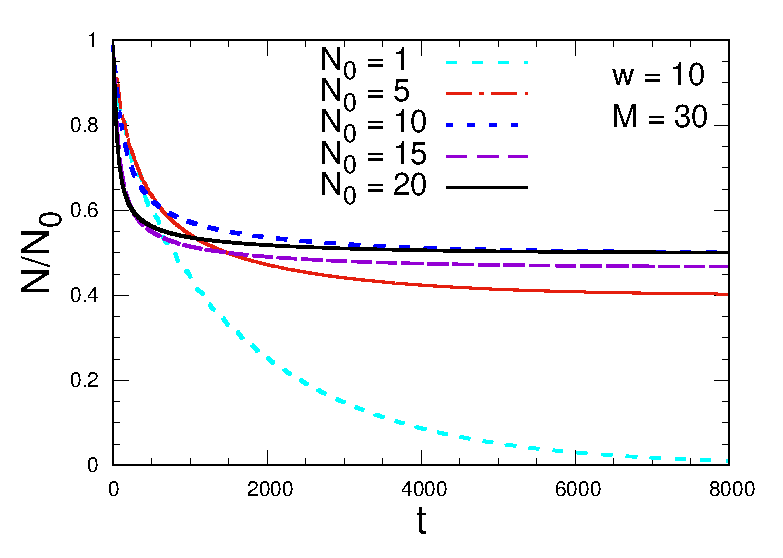
\includegraphics[width=0.65\columnwidth]{imm/Now10.eps}
    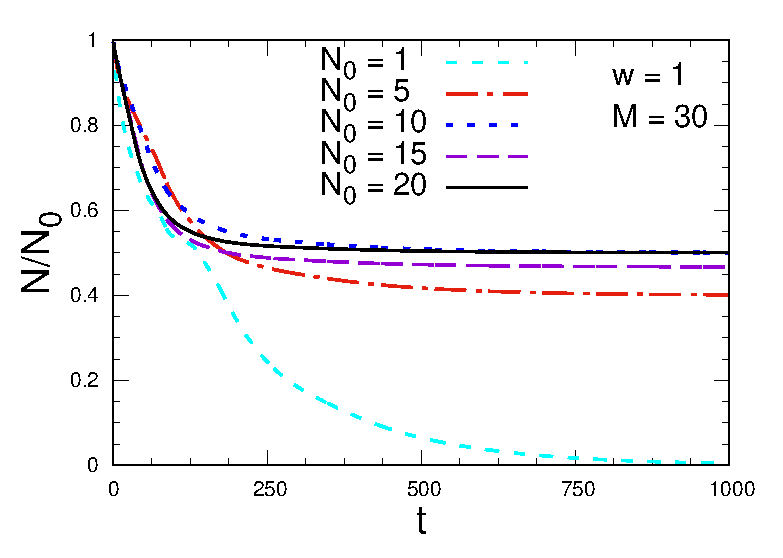
\includegraphics[width=0.65\columnwidth]{imm/No.eps}
    \caption{Behavior of the ratio $N(t)/N_0$ for the central-site
      particle-loss dissipation in systems of size $L=61$ ($M=30$)
      within hard walls, various initial particle number $N_0$, and
      dissipation localized at the center of the system, with $w=1$
      (bottom) and $w=10$ (top).  In both cases asymptotic stationary
      limit turns out to converge to $N/N_0=1/2$ for even $N_0$, and
      $N/N_0=(N_0-1)/(2N_0)$ for odd $N_0$.  Note that approach to the
      asymptotic value is slower for $w=10$ than $w=1$.}
    \label{ndiffn0}
  \end{figure}
  
  
  
  If we consider a central-site dissipation, thus $z=M+1=(L+1)/2$ [we
    recall that we are using shifted coordinates with respect to
    Eq.~(\ref{Hfree})], then the condition (\ref{kz}) reduces to $k=2j$,
  thus implying that $n_k$ remains unchanged for all even $k$ (whose
  odd-parity modes vanish at the central dissipative site), while it
  gets suppressed for odd $k$. Therefore, Eq.~(\ref{ddtnk}) implies that
  half of the fermions survives centrally localized decay
  dissipation. More precisely the stationary states are characterized by
  a residual particle number $N_{\rm asy} = N_0/2$ for even $N_0$, and
  $N_{\rm asy} = (N_0-1)/2$ for odd $N_0$.
  
  Note that the particle loss localized at the center, preserving the
  parity symmetry with respect to the center of the chain, is the
  optimal one to keep a fraction of fermionic particles at large time.
  For example, in the case of a dissipation at the boundaries, i.e.,
  when $z=1$ or $z=M$ in Eq.~(\ref{ddtnk}), no particles survive because
  all $k$-modes are involved by the Lindblad operator, leading to the
  complete suppression of the particles filling the initial ground
  state.
  
  \begin{figure}[!htb]
\centering
    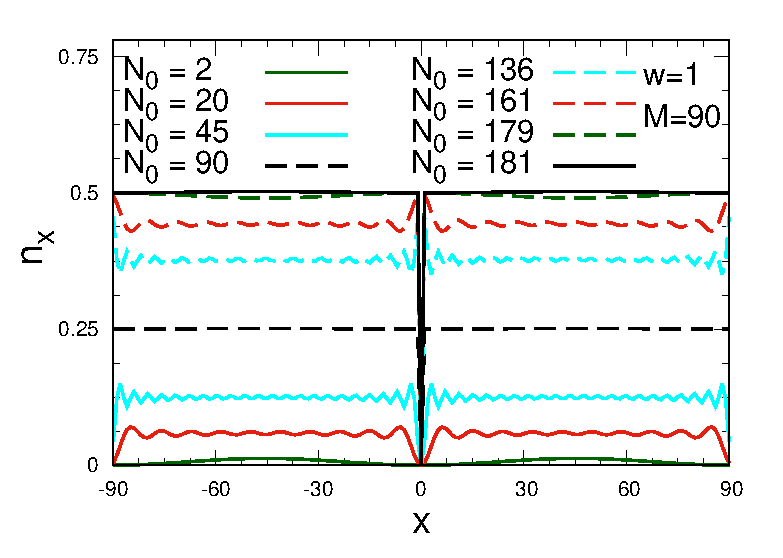
\includegraphics[width=0.65\columnwidth]{imm/nxhwall.eps}
    \caption{Data for the quantum evolution of the fermionic gas within
      hard walls, size $L=2M+1$ with $M=90$, initial particle number
      $N_0=10$, dissipation localized at the center of the chain with
      $w=1$. We show the particle density $n_x(t)$ at the sites $x=0$
      and $x=10$ (top), and the ratio $N(t)/N_0$ (bottom).  They
      approach asymptotic stationary limits (at least within the
      numerical precision, which is very accurate).}
    \label{nxdiffn0time}
  \end{figure}

  
  \begin{figure}[!htb]
\centering
    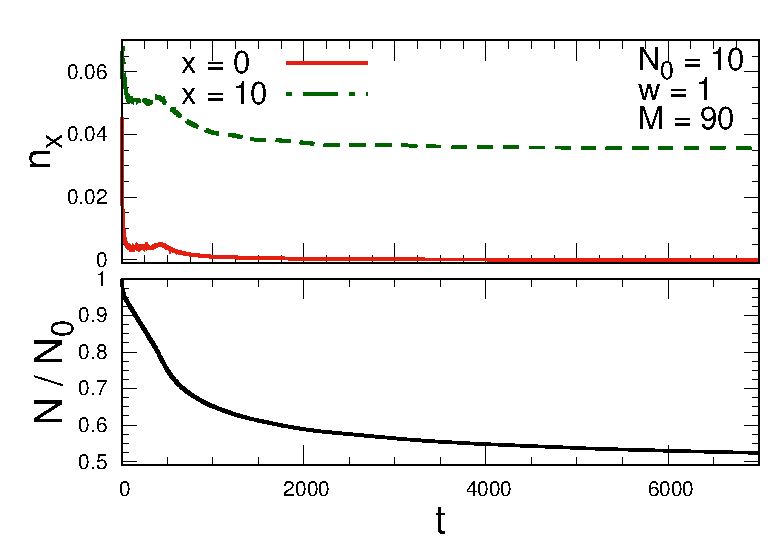
\includegraphics[width=0.65\columnwidth]{imm/nxNo.eps}
    \caption{Asymptotic stationary limit of the particle density $n_x$
      for systems of size $L=181$ ($M=90$) within hard-wall boundary
      conditions, in the presence of a central-site dissipation with
      $w=1$, and for various $N_0$. In all cases the particle density
      vanishes for $x=0$, and it is almost flat elsewhere, apart from
      small spatial oscillations, which appear similar to the
        Friedel oscillations characterizing the behavior of closed
        particle systems}.
    \label{nxdiffn0}
  \end{figure}
  
  
  The above analytical results are confirmed by the numerical results
  for the central particle-loss dissipation, see for example
  Fig.~\ref{ndiffn0} where we show the time dependence of the ratio
  $N(t)/N_0$ for various values of $N_0$ and $w$, and in particular the
  approach to its nonzero asymptotic limit. Also the space dependence of
  the particle density $n_x$ turns out to become stable asymptotically,
  approaching a stationary configuration, as shown in
  Fig.~\ref{nxdiffn0time}.  In Fig.~\ref{nxdiffn0} we show some results
  for the spatial dependence of the average particle density $n_x$ of
  the asymptotic stationary states. We note that $n_x$ is quite flat
  except at $x=0$ where the dissipative mechanism acts, and at the
  boundaries of the chain (essentially due to the hard-wall boundary
  conditions). The almost flat region shows some spatial oscillations,
  which appear suppressed when $N_0\approx M$ and $N_0\approx 2M$.
  
  
  \subsection{Approach to the asymptotic states}
  \label{asyappro}
  
  
  \subsubsection{Large-size behavior of the Liouvillian gap}
  \label{liogap}
  
  
  
  The approach to the stationary state is controlled by the Liouvillian
  gap $\Delta_{\cal L}$ of the generator ${\cal L}$ of the Lindblad
  equation~\cite{BP-openquantumsystembook,RH-book,Z-2015-relaxtimes,MBBC-18,KS-2020-boundarydephasing},
  \begin{equation}
  \Delta_{\cal L} = - {\rm Max}_{i>0} \, {\rm Re}\,(\Lambda_i)\,,
  \label{deltadeb}
  \end{equation}
  where $\Lambda_i$ are the eigenvalues of ${\cal L}$ (we recall that
  the largest eigenvalue is $\Lambda_0=0$ and ${\rm Re} \,\Lambda_i<0$
  for any $i>0$).  The Liouvillian gap for homogeneous spin chains and
  fermionic wires with localized dissipative mechanisms, such as that
  described by Eq.~(\ref{Lindop}), shows generally the asymptotic
  finite-size
  behavior~\cite{PP-08,P-2008-thirdquantization,Z-2015-relaxtimes,KS-2020-boundarydephasing,TV-2021-dissipativeboundaries}
  \begin{equation}
  \Delta_{\cal L}(w,L)\approx D_{\cal L}(w) \,L^{-3}\,.  
  \label{deltaL}
  \end{equation}
  We expect that this asymptotic large-$L$ behavior holds independently
  of the location of the particle-decay dissipation, and it does not
  depend on the initial conditions, thus on $N_0$.  The scaling equation
  (\ref{deltaL}) implies that the approach to the asymptotic behavior
  becomes slower and slower with increasing the size $L$ of the lattice
  at fixed $w$.
  
  \begin{figure}[!htb]
\centering
    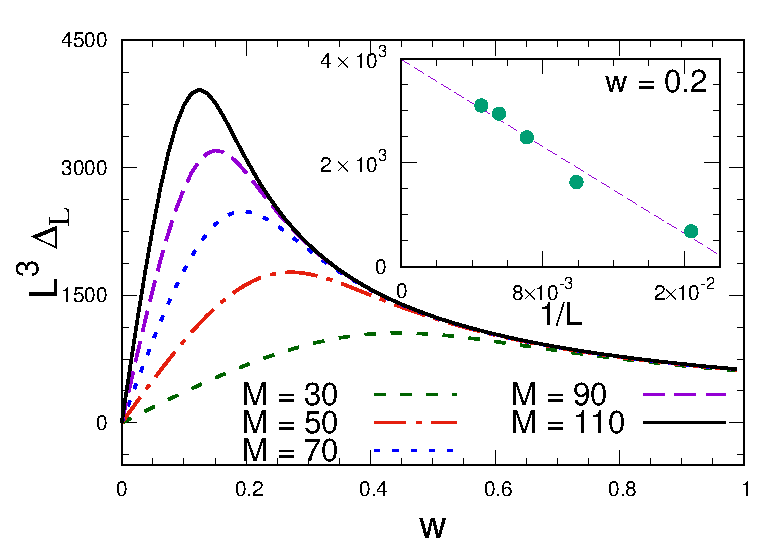
\includegraphics[width=0.65\columnwidth]{imm/DeltawNoL3.eps}
    \caption{The Liouvillian gap $\Delta_{\cal L}$ for particle-decay
      dissipation localized at the center of the chain, for various
      system size $L=2M+1$. The curves appear to converge with
      increasing $M$; this is clearly shown at least for $w\gtrsim 0.2$,
      as also shown by the large-$L$ convergence at a fixed value
      $w=0.2$ [suggesting that the corrections to the asymptotic scaling
      behavior (\ref{deltaL}) are approximately $O(L^{-1})$].  Like the
      case of dissipation at the boundaries, we believe that the
      convergence extends to any $w>0$, but, unlike dissipation at the
      boundaries, it is nonuniform when decreasing $w$ toward zero, see
      text.} 
    \label{liogaps}
  \end{figure}
  
  
  \begin{figure}[!htb]
\centering
    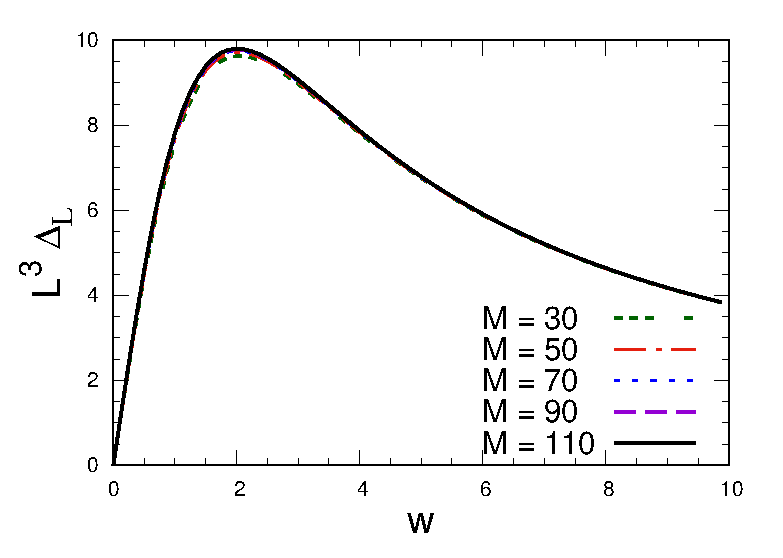
\includegraphics[width=0.65\columnwidth]{imm/deltaextr.eps}
    \caption{Scaling behavior of the Liouvillian gap $\Delta_{\cal L}$
      for particle-decay dissipation localized at one of the boundaries
      of the chain.}
        \label{liogapsb}
  \end{figure}
  
  
  
  
  \begin{figure}[!htb]
\centering
      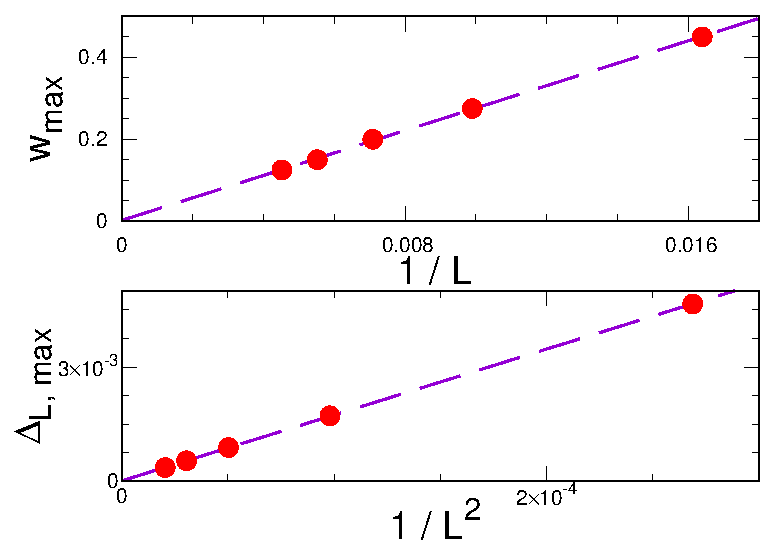
\includegraphics[width=0.65\columnwidth]{imm/wDmax1.eps}
    \caption{Some details of the behavior of the Liouvillian gap
      $\Delta_{\cal L}$ for dissipation localized at the center of the
      lattice. We show the location $w_{\rm max}$ of the maximum of the
      Liouvillian gap (top), showing that $w_{\rm max}\sim L^{-1}$, and
      value of $\Delta_{\cal L}$ at the maximum (bottom), showing that
      $\Delta_{\cal L}(w_{\rm max})\sim L^{-2}$.}
    \label{gapcenterdetails}
  \end{figure}
  
  
  \begin{figure}[!htb]
\centering
    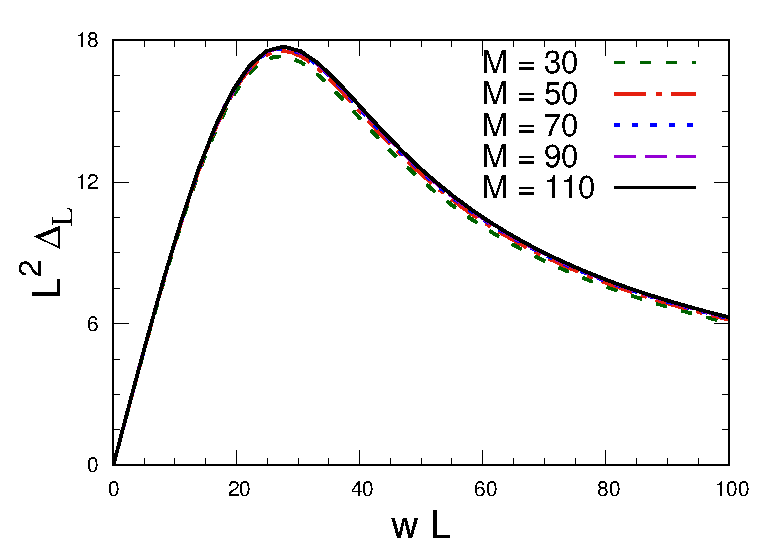
\includegraphics[width=0.65\columnwidth]{imm/DeltawLNo.eps}
    \caption{Plots of $L^2 \Delta_{\cal L}$ versus $wL$ for systems
      within hard walls and with central particle-loss dissipation, for
      various $L=2M+1$.  They support the scaling equation
      (\ref{deltaLcenter}).}
        \label{gapcenter2}
  \end{figure}
  
  The asymptotic behavior (\ref{deltaL}) is confirmed by numerical
  analyses of the Liouvillian gap using the method outlined in
  Ref.~\cite{PP-08}, see App.~\ref{appa}. Some numerical results are
  shown by Figs.~\ref{liogaps} and \ref{liogapsb}, for particle-decay
  dissipation localized at the center and at the boundary of the chain,
  respectively.
  
  In both cases, $\Delta_{\cal L}$ appears nonmonotonic, increasing for
  small values of $w$ and decreasing for sufficiently large dissipation
  strength $w$, for any $L$.  The approach to the asymptotic behavior
  becomes slower and slower with increasing $w$ for large $w$. In
  particular, $\Delta_{\cal L}(w,L)$ shows the large-$w$ behavior $L^3
  \Delta_{\cal L}(w)\approx D_{\cal L}(w)\sim w^{-1}$. This explains the
  results shown in Fig.~\ref{ndiffn0}, where the approach to the
  asymptotic value of the particle number for $w=10$ turns out to be
  slower than that for $w=1$.  The suppression in the limit of
    strong dissipation, for large $w$, may be interpreted as a
    quantum-Zeno-like phenomenon~\cite{MS-1977-quantumzeno,FP-08}, where a strong
    dissipation somehow slows down the dynamics, see
    e.g. Refs.~\cite{TNDTT-17,DMSD-20} for the appearence of similar
    quantum Zeno regimes.
  
  As shown by Figs.~\ref{liogaps} and \ref{liogapsb}, the Liouvillian
  gap at fixed $L$ has a maximum at an intermediate value of
  $w$. The corresponding values $w_{\rm max}$ and $L^3 \Delta_{\cal
      L}(w_{\rm max})$ appears to rapidly converge to the large-$L$
    limit in the case of dissipations localized at the boundaries, but
    they show an apparent size dependence in the case of dissipation
    localized at the center. Indeed the approach to the asymptotic
    $L^{-3}$ behavior (\ref{deltaL}) appears significantly slower in the
    case of dissipation localized at the center, in particular for small
    $w$, which suggests a nonuniform convergence for $w\to 0$.  The
    curves for different lattice sizes appear to clearly converge for
    $w\gtrsim 0.2$, as also shown by the inset of Fig.~\ref{liogaps}. We
    conjecture that, like the case of dissipation at the boundaries, the
    convergence in the large-size limit extends to any $w>0$, but it is
    nonuniform when decreasing $w$ toward zero, unlike dissipation at
    the boundaries.  This is demonstrated by the plots reported in
  Figs.~\ref{gapcenterdetails}, which show that the location of the
  maximum value of the Liouvillian gap for central dissipation moves
  toward $w=0$, with $w_{\rm max}\sim L^{-1}$, and its maximum value
  decreases as $\Delta_{\cal L}(w_{\rm max})\sim w_{\rm max}^2\sim
  L^{-2}$, instead of the general asymptotic $L^{-3}$ behavior for $w>0$
  fixed. Actually, they suggest that the Liovillian gap for central
  dissipation shows also the asymptotic scaling behavior
  \begin{equation}    
  \Delta_{\cal L}(w,L)\approx {\cal D}_{\cal L}(wL) \,L^{-2}\,,
  \label{deltaLcenter}
  \end{equation}
  obtained in the large-$L$ limit keeping $wL$ constant.  This scaling
  behavior is demonstrated by the plot reported in
  Fig.~\ref{gapcenter2}.  Therefore the function $D_{\cal L}(w)$
  entering the asymptotic $L^{-3}$ behavior (\ref{deltaL}) must be
  singular for $w\to 0$ in the case of central-site dissipation,
  diverging as $w^{-1}$.
  
  Note that the above considerations on the behavior of the Liouvillian
  gap apply to generic values of $w$, and,  of course, they do not depend
  on the initial number $N_0$ of particles.  In the following we will
  mainly present results for the value $w=1$ of the dissipation
  parameter, whose dynamic scenarios are shared with those arising from
  generic finite values of $w$.
  
  \subsubsection{Large-time behavior of the particle number}
  \label{lasypgap}
  
  On the basis of the large-size behavior of the Liouvillian gap, we
  expect that the time scale $t_a$ of the approach to the stationary
  state is given as
  \begin{equation}
  t_a \sim \Delta_{\cal L}^{-1}\sim L^3\,,
  \label{timescaleasy}
  \end{equation}
  at fixed $w>0$. This time scale must characterize the approach to the
  stationary limits of the particle number and density.  This is
  confirmed by the numerical computations, see for example
  Fig.~\ref{rntn010} where we report results for the ratio
  \begin{equation}
    R_N(t)\equiv {N(t)-N_{\rm asy}\over N_0-N_{\rm asy}}\,,
      \label{defqu}
  \end{equation}
  for protocols starting from a fixed number $N_0$ of particles.  They
  show the asymptotic large-$L$ scaling behavior
  \begin{eqnarray}
    R_N(t,w,L) \approx A(t/L^3,w)\,,\label{scalbehasy}
  \end{eqnarray}
  which also implies
  \begin{eqnarray}
  {d R_N(t,w,L)\over dt} &\approx& L^{-3} B(t/L^3,w)\,.  \nonumber
  \end{eqnarray}
  Analogous results are obtained for the case we start from a fixed
  ratio $N_0/M$, as shown in Fig.~\ref{dntln0lasy} for $N_0/M=1/2$,
  where we plot $N(t)-N_{\rm asy}$ versus $t/L^3$ and the curves appear
  to collapse in the large-$M$ limit. Note that when $N_0/M$ is kept
  fixed, the quantity $R_N$ defined in Eq.~(\ref{defqu}) is not
  appropriate, because it is always suppressed in the large-time limit,
  due to the denominator that behaves as $N_0-N_{\rm asy}\sim L$.
  
  
  \begin{figure}[!htb]
\centering
    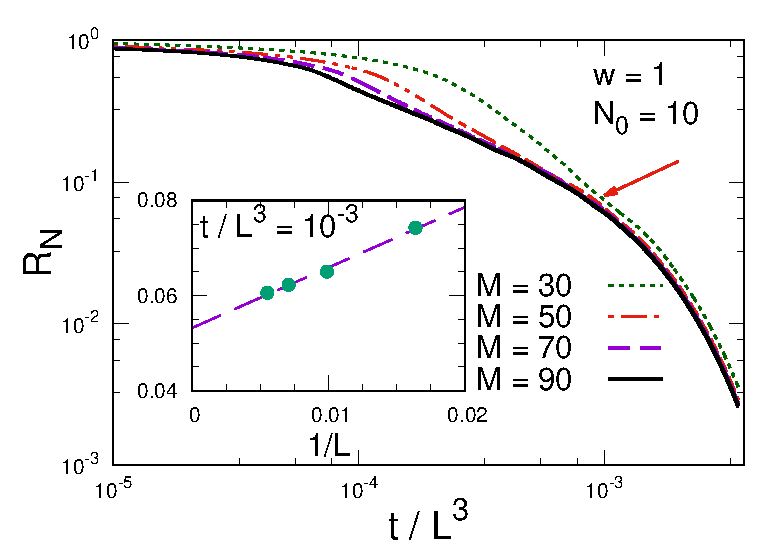
\includegraphics[width=0.65\columnwidth]{imm/NL3.eps}
    \caption{The time dependence of the ratio $R_N$ versus $t/L^3$
      ($L=2M+1$), for homogenous systems within hard walls with $N_0=10$
      and central particle-loss dissipation with $w=1$.  The data for
      various sizes $M$ show clearly the convergence toward a dynamic
      scaling curve, approximately as $1/L$ as shown by the inset for a
      particular value of the ratio $t/L^3$ (the one indicated by the
      arrow in the main figure).}
    \label{rntn010}
  \end{figure}
  
  
  \begin{figure}[!htb]
\centering
    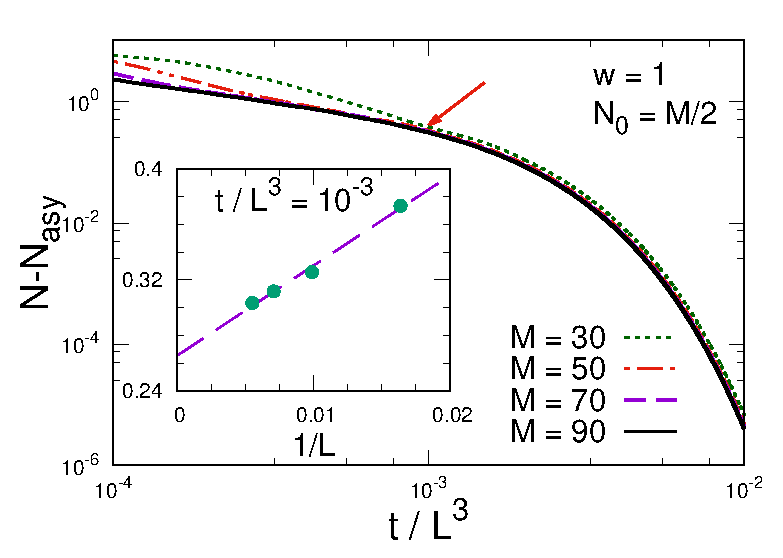
\includegraphics[width=0.65\columnwidth]{imm/dNLL3.eps}
    \caption{The difference $N(t) - N_{\rm asy}$ vs $t/L^3$, for systems
      within hard walls with $N_0/M=1/2$, and central dissipation with
      $w=1$.  Again we observe the asymptotic convergence toward a
      dynamic scaling curve, as shown by the inset for a particular
      value of $t/L^3$ (indicated by the arrow in the main figure).}
    \label{dntln0lasy}
  \end{figure}
  
  As we will show below, this is not the end of the story, indeed
  further peculiar intermediate scaling behaviors emerge, differing
  between the cases $N_0$ and $N_0/M$ fixed.
  
  
  
  
  \subsection{Intermediate scaling behaviors keeping $N_0$ fixed}
  \label{N0fixed}
  
  \begin{figure}[!htb]
\centering
    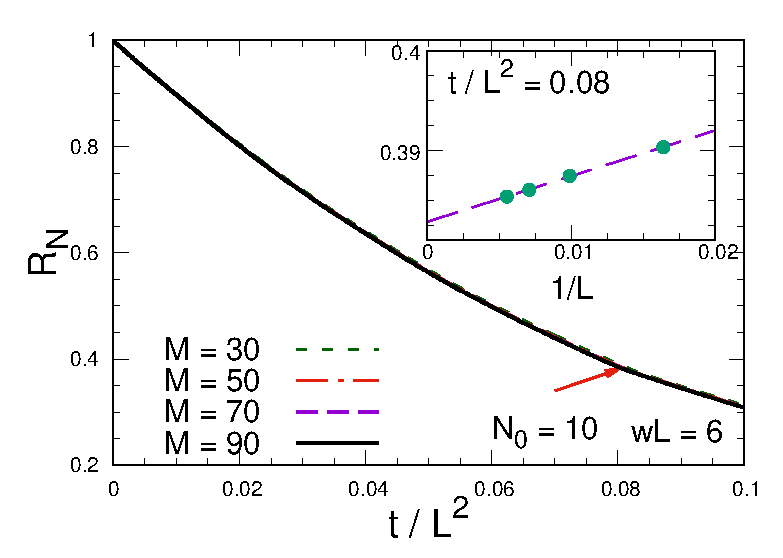
\includegraphics[width=0.65\columnwidth]{imm/NwL2.eps}
    \caption{The ratio $R_N$ versus $t/L^2$ for systems within hard
      walls with $N_0=10$, central dissipation with $wL=6$, for various
      lattice sizes $L=2M+1$.  The data appear to converge toward a
      scaling curve in the large-$L$ limit, as demonstrated by the data
      reported in the inset for a particular value of the ratio
      $t/L^2$.}
    \label{rntn010ir}
  \end{figure}
  
  We now look for intermediate regimes of the time evolution, somehow
  associated with the time scales of the Hamiltonian (\ref{Hfree})
  driving the unitary dynamics, and therefore to its gap $\Delta_H$,
  i.e. the energy difference between the first excited state and the
  ground state. When keeping the particle number $N_0$ fixed, $\Delta_H$
  behaves asymptotically as $\Delta_H \sim L^{-2}$, corresponding to the
  dynamic exponent $z=2$ of the vacuum-superfluid
  transition~\cite{S99}.
  
  We want to check whether the
    out-of-equilibrium dynamics develops an intermediate regimes somehow
    controlled by the Hamiltonian driving of the Lindblad equation,
    whose intrinsic time scale is related to its gap, i.e. $t \sim
    \Delta_H^{-1}\sim L^2$, which is much smaller than the time scale
    $t\sim L^3$ characterizing the approach to the stationary large-time
    limit (of course, for sufficiently large $L$, and in particular in
    the large-$L$ limit). As we shall see, a closer look at the time
    evolution provides a clear evidence of such intermediate regime, which 
     also requires a rescaling of the dissipation strength.
  
  
  In Fig.~\ref{rntn010ir} we show some results for the time dependence
  of the particle number in the case of systems with central-site
  dissipation starting from a fixed number of particles. We observe that
  the above-mentioned intermediate regime exists, and extends to any
  $t\sim L^2$, if we perform an appropriate rescaling of the dissipation
  parameter $w$, decreasing $w$ as $w\sim L^{-1}$. Indeed the numerical
  results clearly support the large-$L$ scaling behavior
  \begin{eqnarray}
   R_N(t,w,L) \approx U(t/L^2,wL)\,,   \label{scalbehwl}
  %%  L^2 {d R_N(t,w,N_0,L)\over dt} &\approx& W(t/L^2,wL)\,,\nonumber
  \end{eqnarray}
  which is obtained by increasing $L$ keeping the ratio $t/L^2$ and the
  product $wL$ fixed.  Note that this intermediate scaling behavior is
  expected to hold even for large values of the ratio $t/L^2$, because
  it is also compatible with the alternative scaling behavior
  (\ref{deltaLcenter}) of the Liouvillian gap.
  
  
  
  
  
  
  \subsection{Intermediate dynamic behavior keeping $N_0/M$ fixed}
  \label{N0oLfixed}
  
  \begin{figure}[!htb]
\centering
    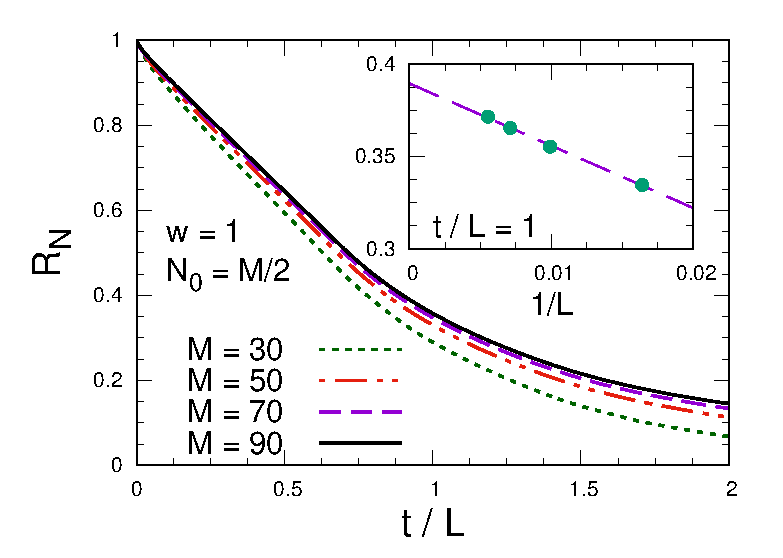
\includegraphics[width=0.65\columnwidth]{imm/NLL1.eps}
    \caption{Behavior of the ratio $R_N$ versus $t/L$, for systems
      within hard walls with $N_0/M=1/2$, and central dissipation with
      $w=1$. The inset shows the $1/L$ approach to the large-$L$
      asymptotic behavior.}
    \label{rntn0lvstol}
  \end{figure}
  
  We now consider the large-$L$ behavior in the case we keep the ratio
  $N_0/M$ fixed when increasing $L=2M+1$. This corresponds to the
  superfluid phase, i.e. when the chemical potential $\mu$ is larger
  than that at the vacuum-superfluid transition, $\mu>-2$. Within the
  superfluid phase, the gap $\Delta_S$ of isolated free Fermi gases
  behaves as~\cite{S99} $\Delta_S \sim L^{-1}$.
  
  Again we want to check whether the out-of-equilibrium dynamics in
    this condition develops an intermediate regime controlled by the
    part of the Lindblad equation driving the unitary dynamics
    introduces a time scale $t\sim \Delta_S^{-1}\sim L$ (again, much
    smaller than the time scale $t\sim L^3$ characterizing the approach
    to the stationary large-time limit). Like the case at fixed $N_0$,
    we show that such an intermediate regime exists.
  
  The existence of a corresponding intermediate regime of the dynamics
  is demonstrated by the results shown in Fig.~\ref{rntn0lvstol},
  leading to the intermediate scaling ansatz
  \begin{eqnarray}
   R_N(t,w,L) \approx W(t/L,w)\,,   \label{scalbehnol}
  %%  L {d R_N(t,w,L)\over dt} &\approx& W(t/L,w)\,,\nonumber
  \end{eqnarray}
  obtained keeping $t/L$ fixed in the large-$L$ limit.  
  
  We finally report the existence of a further early-time regime when we
  start from the ground state for $N_0\propto M$, as already noted in
  Ref.~\cite{FMKCD-20}. Indeed, for sufficiently small time
  \begin{equation}
    {d N(t,w,L)\over dt} \approx  f(t,w)\,,
    \label{vereg}
    \end{equation}
  without showing any asymptotic size dependence.  This is shown by the
  curves reported in Fig.~\ref{rntln0lvst}.  The behavior (\ref{vereg})
  is observed in the large-size limit, and can be considered as the {\em
    thermodynamic} limit of the quantum evolution, when the time is
  sufficiently small that the dynamics does not yet detect the effects
  of the boundaries.  Indeed deviations are observed for $t\propto M$,
  thus later and later for larger and larger systems. At the end of this
  early-time regime, the intermediate regime (\ref{scalbehnol}) begins.
  
  
  
  \begin{figure}[!htb]
\centering
  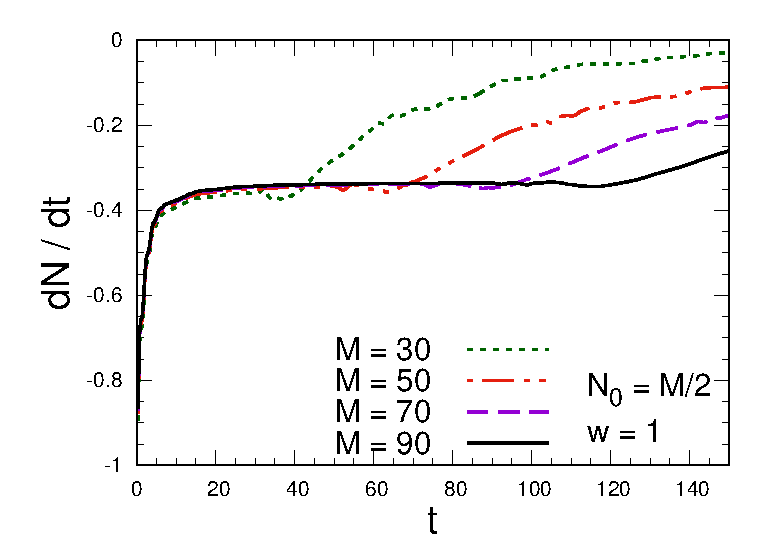
\includegraphics[width=0.65\columnwidth]{imm/dNLL0.eps}
  \caption{The time dependence of the derivative of the particle number,
    for systems within hard walls with central-site dissipation with
    $w=1$, starting from ground states with $N_0/M=1/2$ fixed.  }
    \label{rntln0lvst}
  \end{figure}
  
  
  
  \section{Fermionic gases within harmonic traps}
  \label{hartra}
  
  
  We now present results for lattice fermionic systems within traps
  arising from inhomogeneous external potentials, such as those in
  Eq.~(\ref{potential}), in the presence of a particle-decay dissipation
  at the center of the trap, as described by the Lindblad equations
  (\ref{eqlindblad}) and (\ref{Lindop}). As already mentioned in
    the introductive section, effective harmonic trapping mechanisms are
    quite common in cold-atom experiments~\cite{BDZ-08}. Therefore their
    analysis is also relevant from a phenomonological point of view.
  
  We study the time evolution in the limit of large trap size $L_t$, in
  the case we keep the initial particle number $N_0$ fixed, and when we
  keep the ratio $N_0/L_t$ constant (equivalent to addiing a chemical
  potential). We consider harmonic traps, thus $p=2$ in
  Eq.~(\ref{potential}). The results are obtained for sufficiently large
  systems $L$ at fixed $L_t$, so that a further increases of $L$ does
  not change the results at fixed $L_t$, and therefore they can be
  considered as results for infinite-size systems with a large accuracy,
  within the accuracy of the numerical calculations, better than
  $10^{-8}$.
  
  
  \subsection{Large-time behavior}
  \label{asytrap}
  
  \begin{figure}[!htb]
\centering
    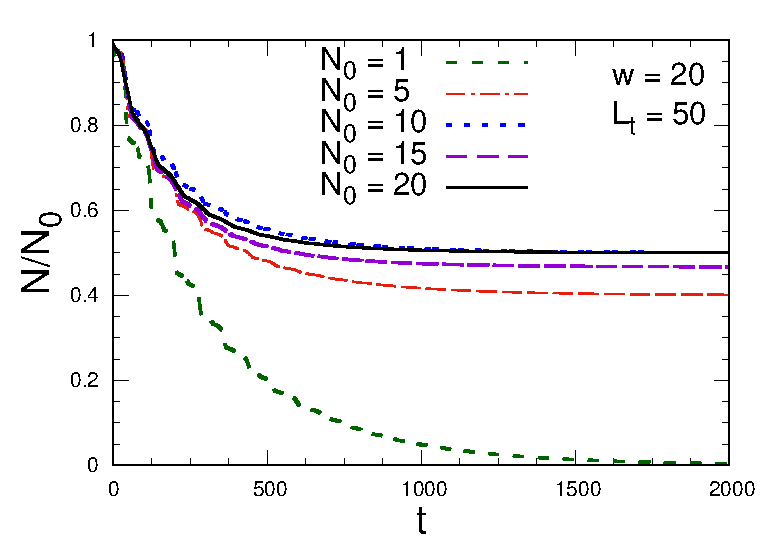
\includegraphics[width=0.65\columnwidth]{imm/trapNow20.eps}
  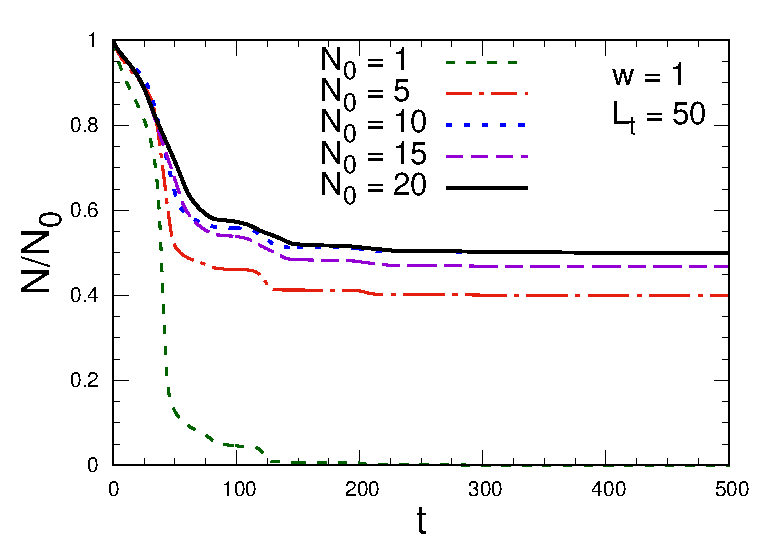
\includegraphics[width=0.65\columnwidth]{imm/trapNo.eps}
  \caption{The time dependence of the ratio $N/N_0$ for the central-site
    particle-loss dissipation $w=1$ (bottom) and $w=20$ (top) in systems
    within harmonic traps, various $N_0$, and $L_t=50$ (in the large-$L$
    limit to make the finite-size effects negligible).  The asymptotic
    stationary limit turns out to converge to $N/N_0=1/2$ for even
    $N_0$, and $N/N_0=(N_0-1)/(2N_0)$ for odd $N_0$. Similarly to the
    case of systems within hard walls, see Fig.~\ref{ndiffn0}, the
    approach to the asymptotic value turns out to be slower for $w=20$
    than $w=1$.}
  \label{traptdep}
  \end{figure}
  
  
  To begin with, we discuss the asymptotic stationary states.  In
  Fig.~\ref{traptdep} we show the time dependence, and asymptotic
  behavior, of the ratio $N(t)/N_0$ for various values of the initial
  number of particles. Again, similarly to the case of homogeneous
  systems within hard walls and particle-decay dissipation at the center
  of the chain, we find that the large-time states keep a half of the
  initial particles.  Analogously to the hard-wall case, this can be
  related to the fact that the one-particle Hamiltonian is invariant
  under reflections with respect to the center, thus the one-particle
  states must have definite parity. This can be easily seen in the
  continuum limit, see e.g. Ref.~\cite{ACV-14}, where the one-particle
  Hamiltonian eigenfunctions can be written in terms of Hermite
  polynomials, and have definite parity.  Since the one-particle states
  with negative parity vanishes at the center of the trap, the
  corresponding modes in the ground state of the fermionic system are
  not affected by the particle-decay dissipation at the center of the
  trap. Then, recalling that the ground state is obtained by filling the
  first $N_0$ one-particle levels, a selection mechanism analogous to
  that identified in the case of homogeneous systems applies, see
  Sec.~\ref{asysta}, therefore half of them are odd [more precisely
    $N_0/2$ for even $N_0$ and $(N_0-1)/2$ for odd $N_0$], we expect
  again that half particles survive the central particle loss.
  
  \begin{figure}[!htb]
\centering
  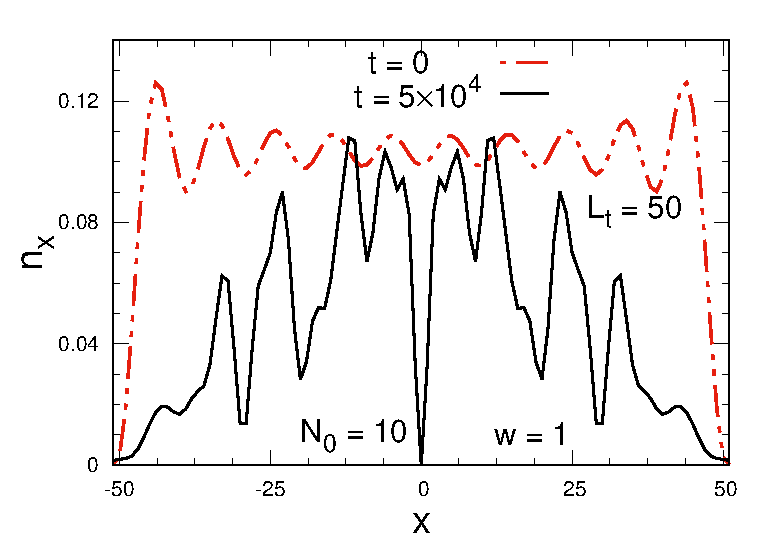
\includegraphics[width=0.65\columnwidth]{imm/trapnxLt50.eps}
  \caption{The particle density $n_x$ for systems within a harmonic trap
    with initial particle number $N_0=10$, at $t=0$ and after some time
    $t$, for a central dissipation with $w=1$, fixed trap size $L_t=50$,
    and for a sufficiently large size of the system, $L=221$, to make
    finite-size effects negligible (numerically checked by verifying the
    dependence on $L$).}
  \label{trapnxt}
  \end{figure}
  
  In Fig.~\ref{trapnxt} we show the particle density at $t=0$ and at
  large time when the central particle density has already stably
  vanished. However, the spatial dependence of the particle density does
  not appear static in the large-time regime where the particle number
  stops decreasing. Indeed, as shown in Fig.~\ref{trapnxto}, the time
  dependence of the particle density at sites $x\neq 0$ is characterized
  by time oscillations that apparently continue indefinitely, persisting
  even in the large-$L_t$ limit.  We also note that in this large-time
  regime the quantum evolution of the particle density appears
  effectively driven by the Hamiltonian term only. We have checked that
  the dissipative contribution in Eq.~(\ref{eqscxytrap}), i.e. the one
  proportional to $w$, gets suppressed asymptotically, thus only the
  Hamiltonian determines the large-time dependence of the fixed-time
  two-point function ${\mathscr C}_{xy}(t)$ and $n_x={\mathscr
    C}_{xx}(t)$. In this large-time regime also the energy of the system
  defined in Eq.~(\ref{enedef}) remains constant, indeed its time
  derivative vanishes when ${\rm Re}\,{\mathscr C}_{0,1}=0$,
  cf. Eq.~(\ref{derene}).
  
  
  
  
  
  
  \begin{figure}[!htb]
\centering
  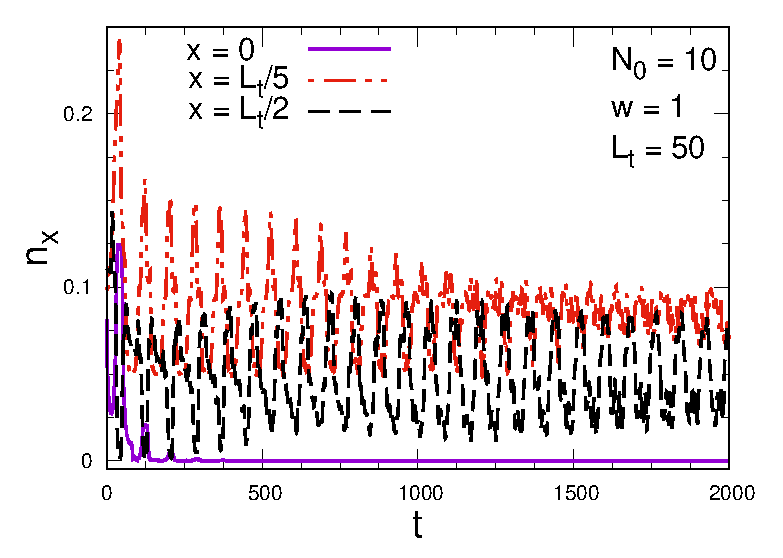
\includegraphics[width=0.65\columnwidth]{imm/nxtLt50.eps}
  \caption{ Time dependence of the particle density for systems within a
    trap of size $L_t=50$, at various spatial coordinates, $x=0$,
    $x=L_t/5=10$ and $x=L_t/2=25$, for central dissipation with $w=1$.
    The particle density $n_x$ for $x\neq 0$ are characterized by
    oscillations in the large-time regime, when $n_x$ at $x=0$ and the
    particle number have already approached their asymptotic behavior.
  }
  \label{trapnxto}
  \end{figure}
  
  
  \subsection{Large-$L_t$ scaling behavior of the time dependence}
  \label{trapscaling}
  
  
  The time dependence starting from a fixed number of particles shows
  the peculiar scaling behavior
  \begin{equation}
    R_N(t,w,L_t) \equiv {N(t)-N_{\rm asy}\over N_0-N_{\rm asy}} \approx
    A_t(t/L_t,w)\,,
    \label{rntrapn0}
  \end{equation}
  which apparently describes the whole time evolution.  This is clearly
  supported by the data reported in Figs.~\ref{trapNo} and
  \ref{trapNow01} for central dissipation with $w=1$ and initial
  particle number $N_0=10$.
  
  Note that the time scale $t\sim L_t$ may be also related to the gap of
  the fermionic Hamiltonian, for which $\Delta_{L_t} \sim
  L_t^{-z\theta}$ where $z=2$ is the dynamic exponent associated with
  the vacuum-to-superfluid transition, and $\theta=1/2$ is the universal
  trap exponent characterizing critical behaviors in the presence of
  trapping potentials~\cite{CV-09,CV-10,ACV-14,rossini2021coherent} [for generic
    power laws of the potential (\ref{potential}), $\theta=p/(p+2)$].
  
  \begin{figure}[!htb]
\centering
  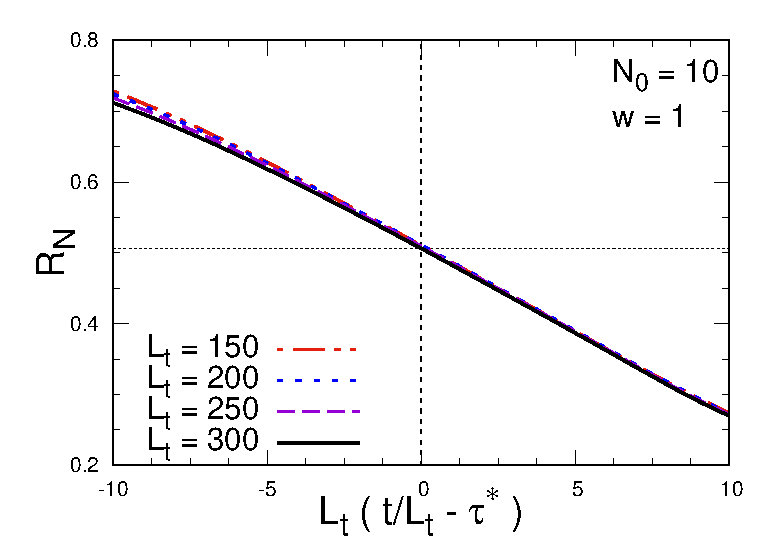
\includegraphics[width=0.65\columnwidth]{imm/crit.eps}
  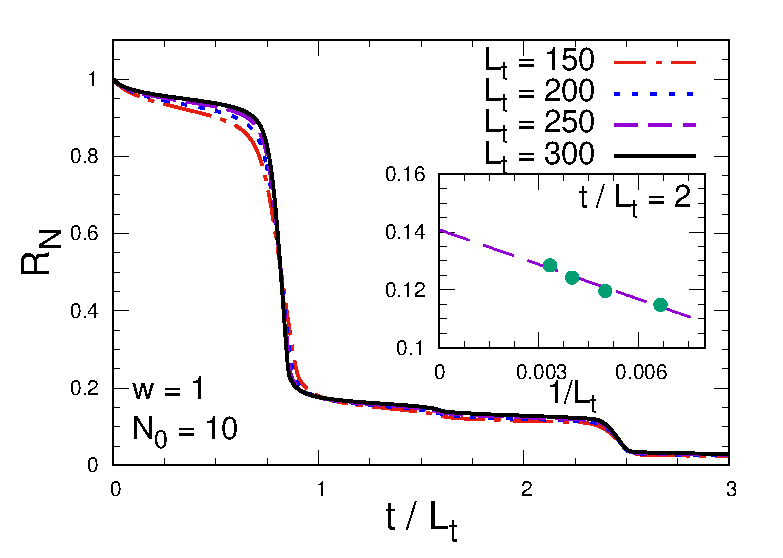
\includegraphics[width=0.65\columnwidth]{imm/RNtrapNo.eps}
  \caption{ The bottom figure shows the time evolution of the ratio
    $R_N$ versus $t/L_t$ for $w=1$, various trap sizes, keeping the
    initial number of particles $N_0=10$ fixed.  The inset shows an
    example of convergence at $t/L_t=2$.  The top figure shows the
    scaling behavior at the fast drop of the particle number, around
    $t/L_t\approx 0.8147$, described by Eq.~(\ref{atcrit}).  }
  \label{trapNo}
  \end{figure}
  
  \begin{figure}[!htb]
\centering
  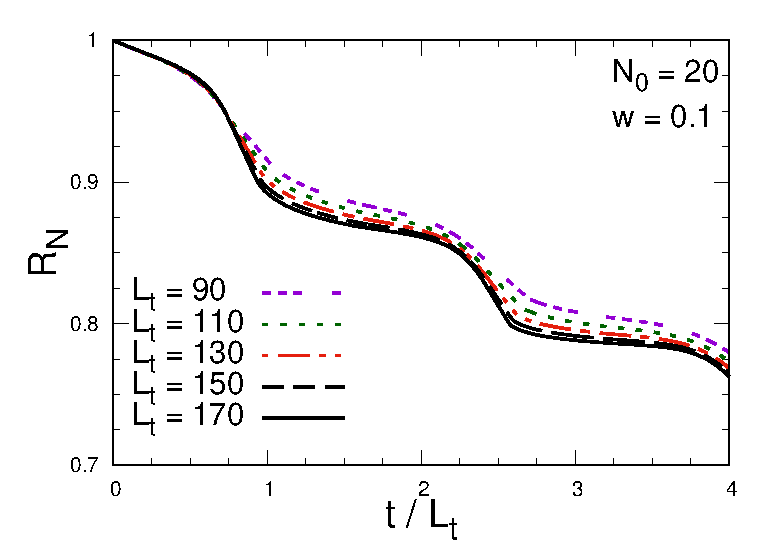
\includegraphics[width=0.65\columnwidth]{imm/RNtrapNo20w01.eps}
  \caption{The ratio $R_N$ for $w=0.1$, various trap sizes, keeping the
    initial number of particles $N_0=20$ fixed.}
  \label{trapNow01}
  \end{figure}
  
  \begin{figure}[!htb]
\centering
  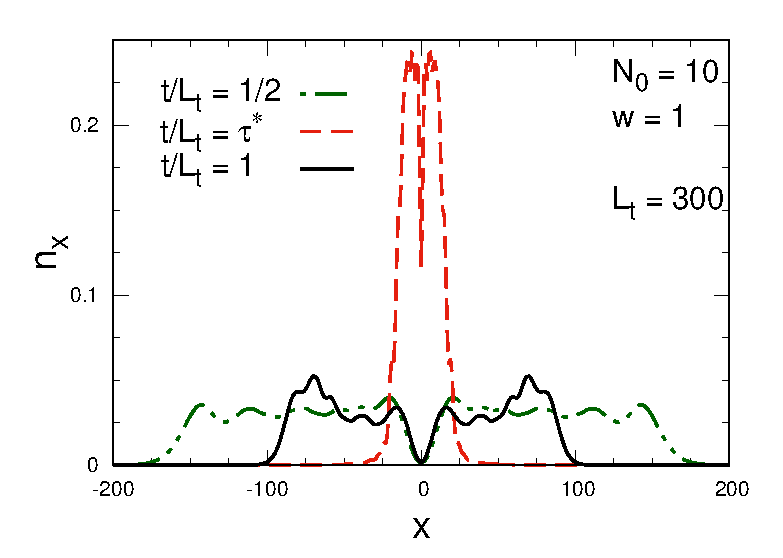
\includegraphics[width=0.65\columnwidth]{imm/nxtrap.eps}
  \caption{ Behavior of the particle density around the singularity of
    the scaling function (\ref{rntrapn0}), for $L_t=300$, central
    particle loss with $w=1$, and some values of the ratio $t/L_t$
    around the singular point $t/L_t =\tau^*\approx 0.8147$. They show
    that large drop of the particle number at $\tau^*$ is connected with
    a simultaneous large increase of the particle density at the center
    of the trap.  }
  \label{trapnx}
  \end{figure}
  
  
  
  
  
  The time scale $t\sim L_t$ characterizes the whole evolution of the
  system, up to the large-time regime, except for some small
  intermediate time intervals. Indeed, the curves shown in the bottom
  Fig.~\ref{trapNo} presents some flat regions followed by rapid
  changes.  Actually a more careful analysis, see, e.g., the top
  Fig.~\ref{trapNo}, shows that the scaling function $A_t(t/L_t,w)$
  entering Eq.~(\ref{rntrapn0}) appears to develop a singularity in the
  large-time limit, at $t/L_t = \tau^*\approx 0.8147$, so that
  \begin{equation}
    A_t(t/L_t,w) \approx f[L_t (t/L_t-\tau^*)]
    \label{atcrit}
  \end{equation}
  around $t/L_t=\tau^*$. Therefore this sharp drop of the particle
  density occurs at a time $t^* \approx L_t \tau^*$ in the large-$L_t$
  limit, and lasts for a finite time interval, i.e. it does not diverge
  when increasing $L_t$.  Some data for the behavior of the particle
  density and number around the time $\tau^*$ are shown in
  Fig.~\ref{trapnx}, where we note the significant increase of the
  particle density around $x=0$ when the singular behavior of the
  scaling function (\ref{rntrapn0}) appears.  Analogous behaviors are
  observed for generic values of $N_0$ and $w$.
  
  
  In the case we keep $N_0/L_t$ fixed, the results show a generic
  scaling behavior in terms of $t/L_t$, analogous to
  Eq.~(\ref{rntrapn0}), see for example Fig.~\ref{trapNoLt}.
  
  
  
  
  
  
  \begin{figure}[!htb]
\centering
  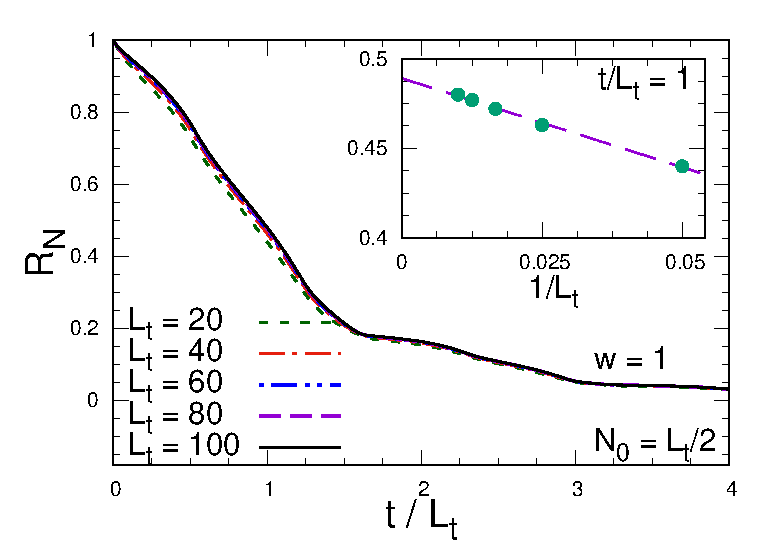
\includegraphics[width=0.65\columnwidth]{imm/RNtrapNoLt.eps}
  \caption{ Time evolution of the ratio $R_N$ versus $t/L_t$ for
    fermionic gases within harmonic traps of various size, keeping the
    ratio $N_0/L_t=1/2$ fixed, for central particle-loss dissipation with
    $w=1$. The  large-$L_t$ convergence is evident, as also shown by
    the plot reported within the inset. }
  \label{trapNoLt}
  \end{figure}
  

\section{From local to uniform dissipation: the sunburst model}

%{\bf describe a bit the model and the interplay between uniform and local dissipation 
%regime}

\begin{figure}
    \centering
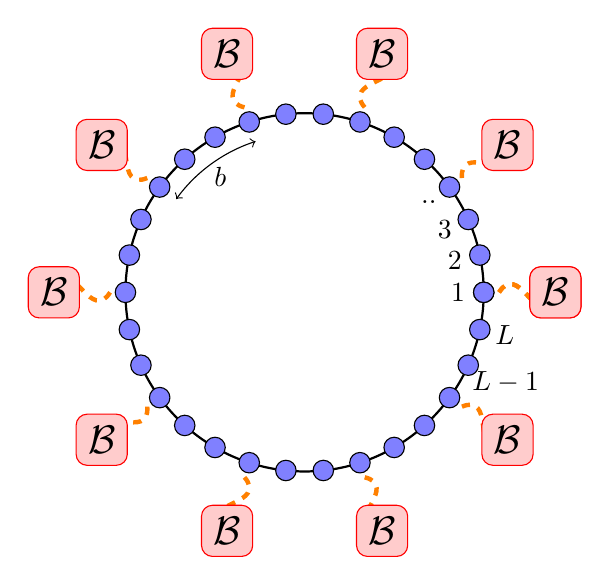
\begin{tikzpicture}[scale=0.65]
    \draw[thick] (0,0) circle (3.5cm);

    \foreach \x in {0,12,...,360}
    \filldraw [fill=blue!50] (\x:3.5cm) circle (0.2);

    \foreach \x in {0,36,...,360}
    \draw[orange, dashed, ultra thick] (\x:3.8cm) .. controls (\x+8:4.2cm) and (\x-8:4.6cm) .. (\x:4.6cm);

    \foreach \x in {0,36,...,360}
    \node[rectangle,
    draw = red,
    text = black,
    fill = red!20!white,
    rounded corners,
    minimum size=0.65cm] (r) at (\x:4.9cm) {\Large $\mathcal{B}$};

    \draw[<->] (108:3.1cm) arc
    [start angle=108,
        end angle=144,
        radius=3.1cm,
    ] ;

    \node[] (s1) at (126:2.8cm) {$b$};

    \node[] (s1) at (0:3cm) {$1$};
    \node[] (s2) at (12:3cm) {$2$};
    \node[] (s3) at (24:3cm) {$3$};
    \node[] (s4) at (36:3cm) {$..$};
    \node[] (s5) at (-12:4cm) {$L$};
    \node[] (s6) at (-24:4.3cm) {$L-1$};
\end{tikzpicture}
    \caption{Sketch of a Kitaev ring with $L=30$ qubits coupled with $n=10$ dissipators in a \textit{sunburst} geometry ($b=3$ in the figure).}
    \label{fig_sketch_sunburst_dissipation}
\end{figure}

We consider a lattice model tailored to unveil the crossover regime between the  dissipation schemes presented. We investigate a $(1+1)$-dimensional Kitaev ring with local particle-decay dissipators arranged in a \textit{sunburst} geometry~\cite{FRV-staticsunburst, FRV-timesunburst, MS-2022-sunburstquench}. The whole apparatus is sketched in Fig.~\ref{fig_sketch_sunburst_dissipation}. The open quantum system is coupled with the environment by means of $n\equiv L/b$ equally-spaced external baths, which reduce to some extent the translation invariance of the starting model.
In particular, we focus on the case of particle-decay jump
operators in the Eq.\eqref{eqlindblad}, i.e., $\hat L_x = \hat c_x$ , where fermionic 
particles are continuously removed from the site $x$. With this choice,
the Liouville operator ${\cal L}$ is quadratic in the fermionic
variables $\hat c_x$ and $\hat c_x^\dagger$ , and, in this sense, we say that the
open ring we study maintains its integrability. Most of
the results discussed in this work should preserve their
validity also for particle-pumping dissipation ( $\hat L_x = c_x^\dagger$ ),
since Eq. \eqref{eqlindblad} is still quadratic in the fermionic creation
and annihilation operators.\\

We explore different large-size limits, depending on the number of dissipators taken into account. A thorough study of the Liouvillian gap $\Delta_\lambda$ is the main focus of the first part of this section. In the second part, we examine the real-time evolution of the system, triggered by a \textit{soft quench} of a coupling constant appearing in the defining hamiltonian~\footnote{In a \textit{soft quench} the variation of the quenched parameter is attenuated down to $0$ with increasing the lattice size $L$.}. Starting the protocol in the proximity of a CQT, we study the out-of-equilibrium dynamic using RG arguments and FSS frameworks~\cite{C-1996-ScalingandRG, RV-2021-coherentanddissipativedynamicsreview}.\\

We emphasize the interplay between the unitary and dissipative dynamics and the role played by the gap $\Delta_\lambda$, extending some of the results already presented in Ref.~\cite{NRV-2019-competingdissipativeandcoherent} to our model. To outline our FSS theory, we mainly focus on the scaling properties of the critical correlations and one of the most common entanglement quantifiers, i.e., the entanglement entropy~\cite{ZMZ-2021-Renyientropiesopen}.



\subsection{Liouvillian Gap}

This section is devoted to discussing the different scaling behaviors observed for the Liouvillian gap $\Delta_\lambda$ defined in the subsection \ref{subsec_liouvilliangap}. We will consider two different limits, depending on the number of dissipation sources considered with increasing the lattice size.

%\vspace{-0.4cm}

\subsubsection{Liouvillian gap at fixed $b$}

The value of the Liouvillian gap at fixed $b$ can be computed using two different algorithm.
One, useful for small value of $b$, consists to analyze the system in the Fourier space 
the Lindblad vectorized Eq. \eqref{vecteqlindblad} whose spectrum gives the gap. 

The latter uses the third quantization technique, see details in 
Ref.~\cite{P-2008-thirdquantization}, particularly convenient for high value of the 
parameter $b$ \cite{franchi2023Liouvillian}. Without loss of generality, we will focus only
on small values of $b$, i.e. up to $b=7$, but all the results can be extended also in
the case of high $b>7$.\\

For $b=3$, the Liouville gap $\Delta_\lambda$ shows a behavior in terms of $w$ in Fig.~\ref{fig_liouvgap3b}.
At fixed $L$, we can easily distinguish two different regimes for the gap, which are separated by a bump in the gap located at $w_*(L)$. We clarify that a non-monotone trend in $\Delta_\lambda$ is not unexpected due to the presence of the \textit{quantum Zeno effect} — the dynamic of a quantum system slows down when it is frequently monitored~\cite{MS-1977-quantumzeno, HHNU-2022-Incoherentons}. Note also that both $w_*(L)$ and $\Delta_\lambda(w_*)$ vanish in the thermodynamic limit, so only the region with $w\geq w_*$ is relevant to determine the typical relaxation time of the system for large enough ring sizes. As shown in Fig.~\ref{fig_liouvgap3b}, for $w<w_*$, the gap is perfectly compatible with a linear dependence of the form

\begin{figure}[!h]
    \centering
    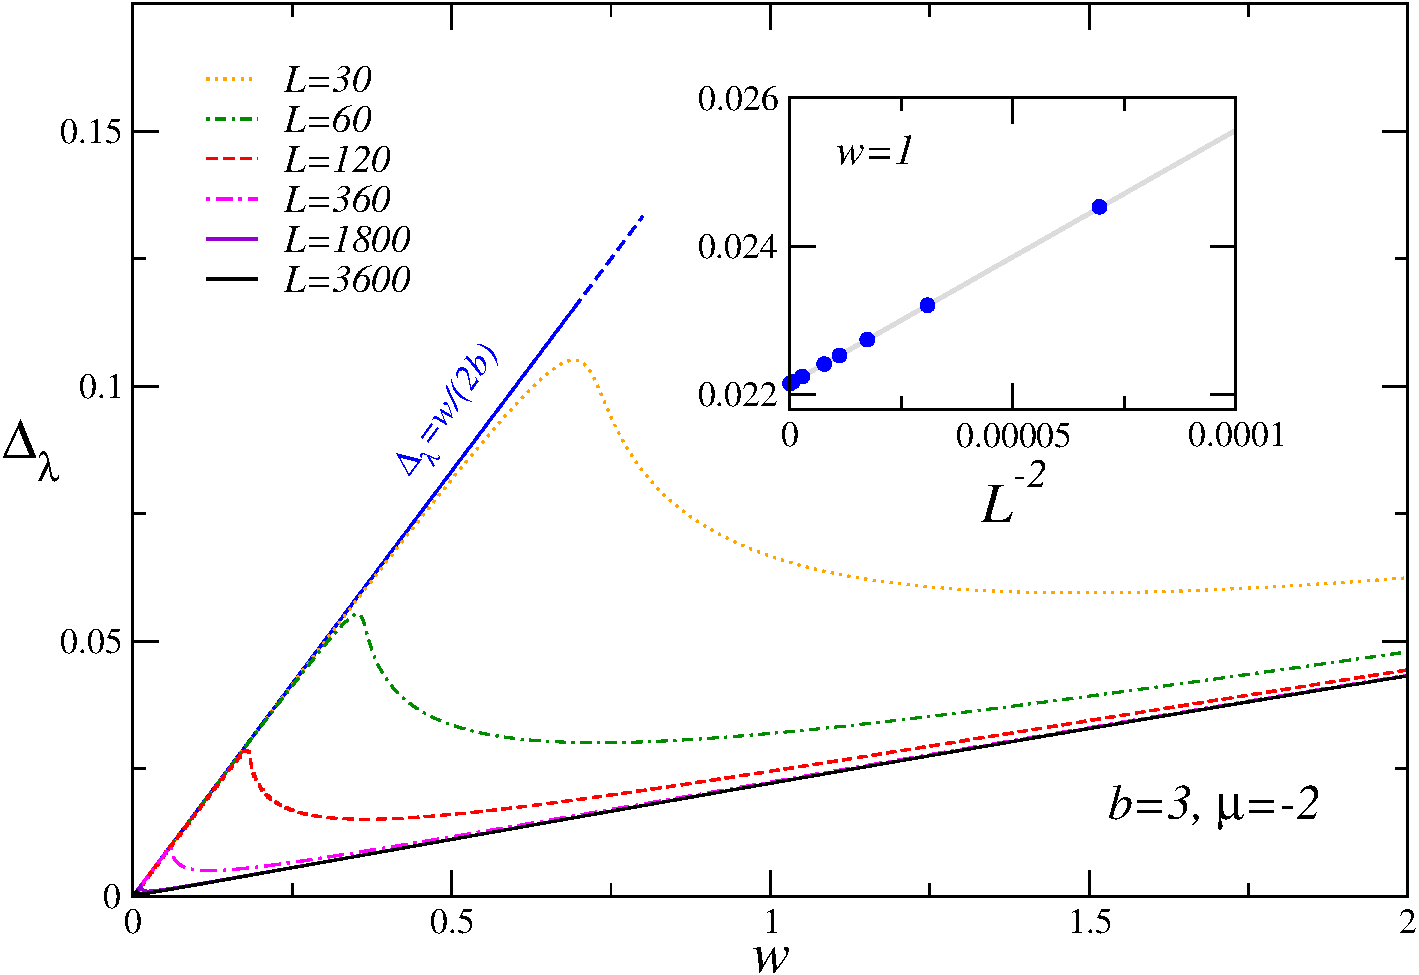
\includegraphics[width=8cm]{imm/gapliouv3b.pdf}
    \caption{Liouvillian gap $\Delta_\lambda$ in terms of the dissipation coupling $w$ for $b=3$ and fixed $\mu=-2$. For small $w$ and $L$ finite, the gap depends linearly on the dissipation strength as $\Delta_\lambda=w/2b$. With increasing $L$ and finite $w>0$, the Liouvillian gap approaches a different regime, which still depends linearly on $w$. In the inset, scaling corrections evaluated at $w=1$ are perfectly consistent with a $L^{-2}$ decaying. The gray straight line is drawn to guide the eye.}
    \label{fig_liouvgap3b}
\end{figure}

\begin{equation}
\Delta_\lambda(w, b)=\frac{w}{2b}\,, \quad w<w_*\,.
\label{eq_deltaL_w_smaller_w*}
\end{equation}

We have verified numerically that the above expression holds also for different values of $b\leq7$ (not shown). This equation has a clear interpretation when we rewrite $\mathbb{D}[\rho]$ in momentum space. Indeed, the full Hilbert space decomposes into the direct product of $n/2$ distinguished sectors with a dimension $4^b$. The effective coupling perceived within each sector is equal to $w/b$. If we additionally assume that the minimum contribution stemming from a single sector is $1/2$ (which is always the case for $b=1$), we get Eq.~\eqref{eq_deltaL_w_smaller_w*}.\\

On the other hand, when $w>w_*$, we observe that the gap $\Delta_\lambda$ still depends linearly on the coupling $w$, but the slope of the asymptotic straight line approached is no longer $1/2b$. We conjecture that for $w>w_*$ and sufficiently large $b$, the following expression describes the Liouvillian gap
\begin{equation}
    \Delta_\lambda(w, b)=A_\mu(b) w\,,\quad A_\mu(b)=\frac{C_\mu}{b^{3}}\,,\quad w>w_*\,,
    \label{eq_liouvillian_gap_largeL}
\end{equation}
where $C_\mu$ is a constant that only depends on the chemical potential $\mu$. Matching arguments with the boundary-dissipation cases surely prompted our guess. Indeed, when $b\propto L$, we expect to recover the leading behavior $\Delta_\lambda\sim L^{-3}$ frequently observed in the literature. Our ansatz is fully supported by the data that we have collected for $A_\mu$ in terms of $1/b^{3}$, as shown in Fig.~\ref{fig_ratelatetime} \footnote{Systematic error bars reported in the figure have been estimated from the comparison of $A_\mu(b)$ for different lattice sizes $L\geq L_{\text{min}}$ and coupling ranges $w\geq w_{\text{min}}$.}. Indeed, a straight line with a slope of $C_\mu=0.601(3)$ describes our data for all values of $b\geq3$ considered ($\chi^2/\text{ndof}=1.0$).  

\begin{figure}
    \centering
    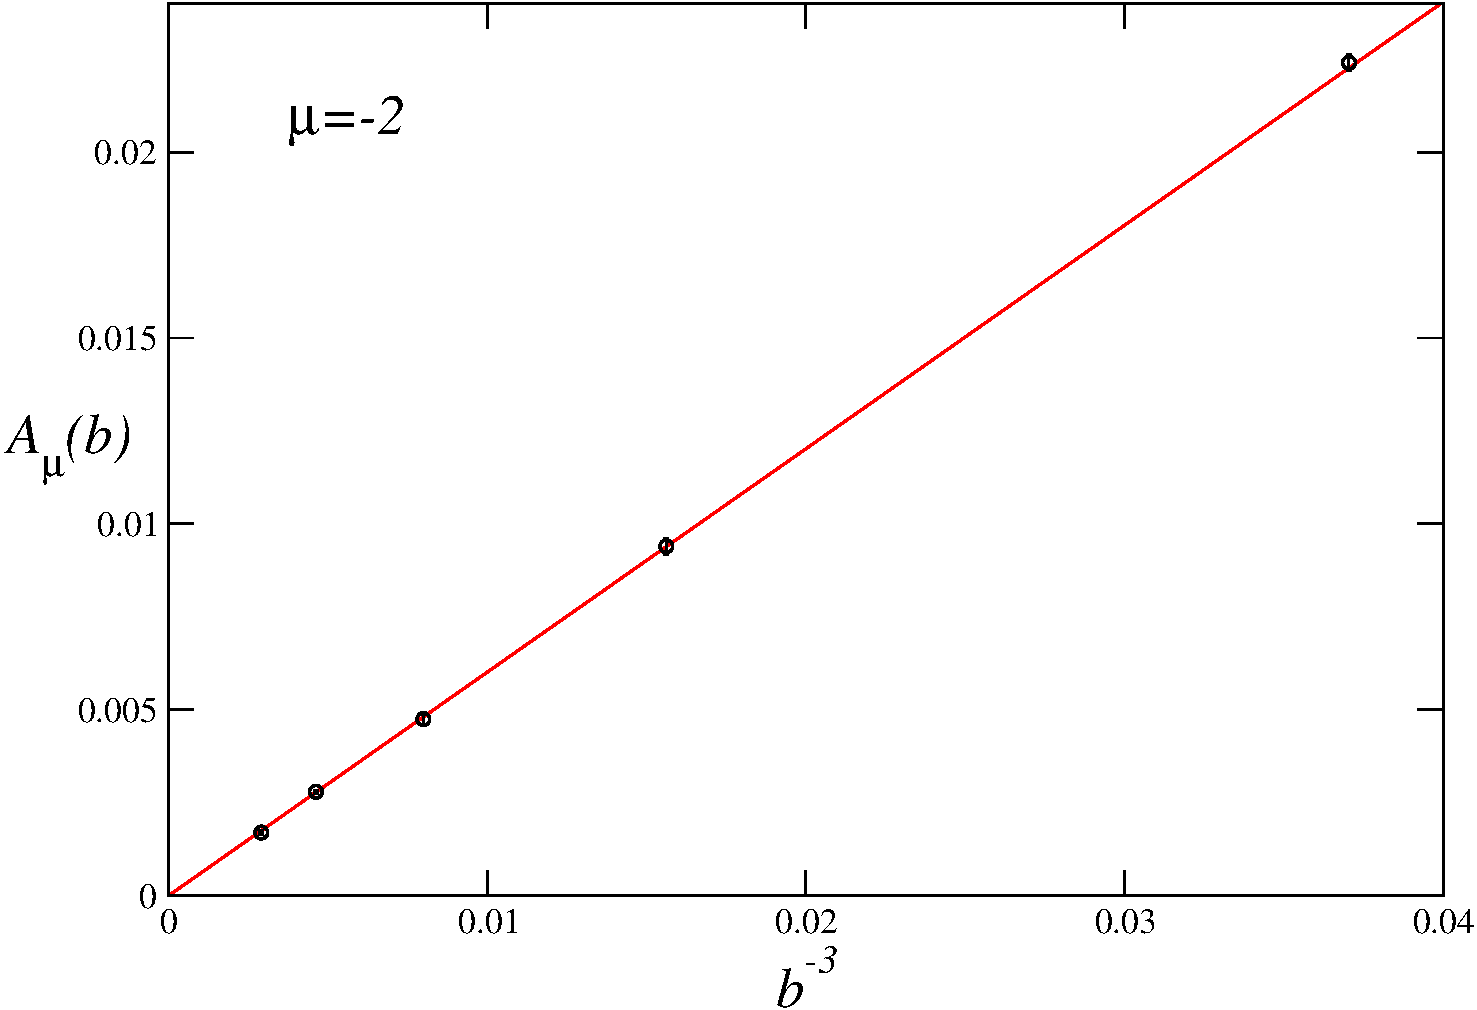
\includegraphics[width=8cm]{imm/ratelatetime.pdf}
    \caption{Liouvillian rate coefficient $A_{\mu}(b)$ versus $b^{-3}$ with constant $\mu=-2$. For $b\geq3$, we observe that $A_{\mu}(b)$ is compatible with a power-law dependence of the form $A_{\mu}(b)=C_{\mu}/b^{3}$, where $C_{\mu}=0.601(3)$ ($\chi^2/\text{ndof}=1.0$).}
    \label{fig_ratelatetime}
\end{figure}

We also want to mention a scaling regime observed for $L\Delta_\lambda$ in terms of $w L$ when the latter quantity is kept fixed in the large size limit. In Fig.~\ref{fig_scaling_delta_apbc}, we report our data for $b=2, \mu=-3$ and $b=4, \mu=-1$.


\begin{figure}[!b]
    \centering
    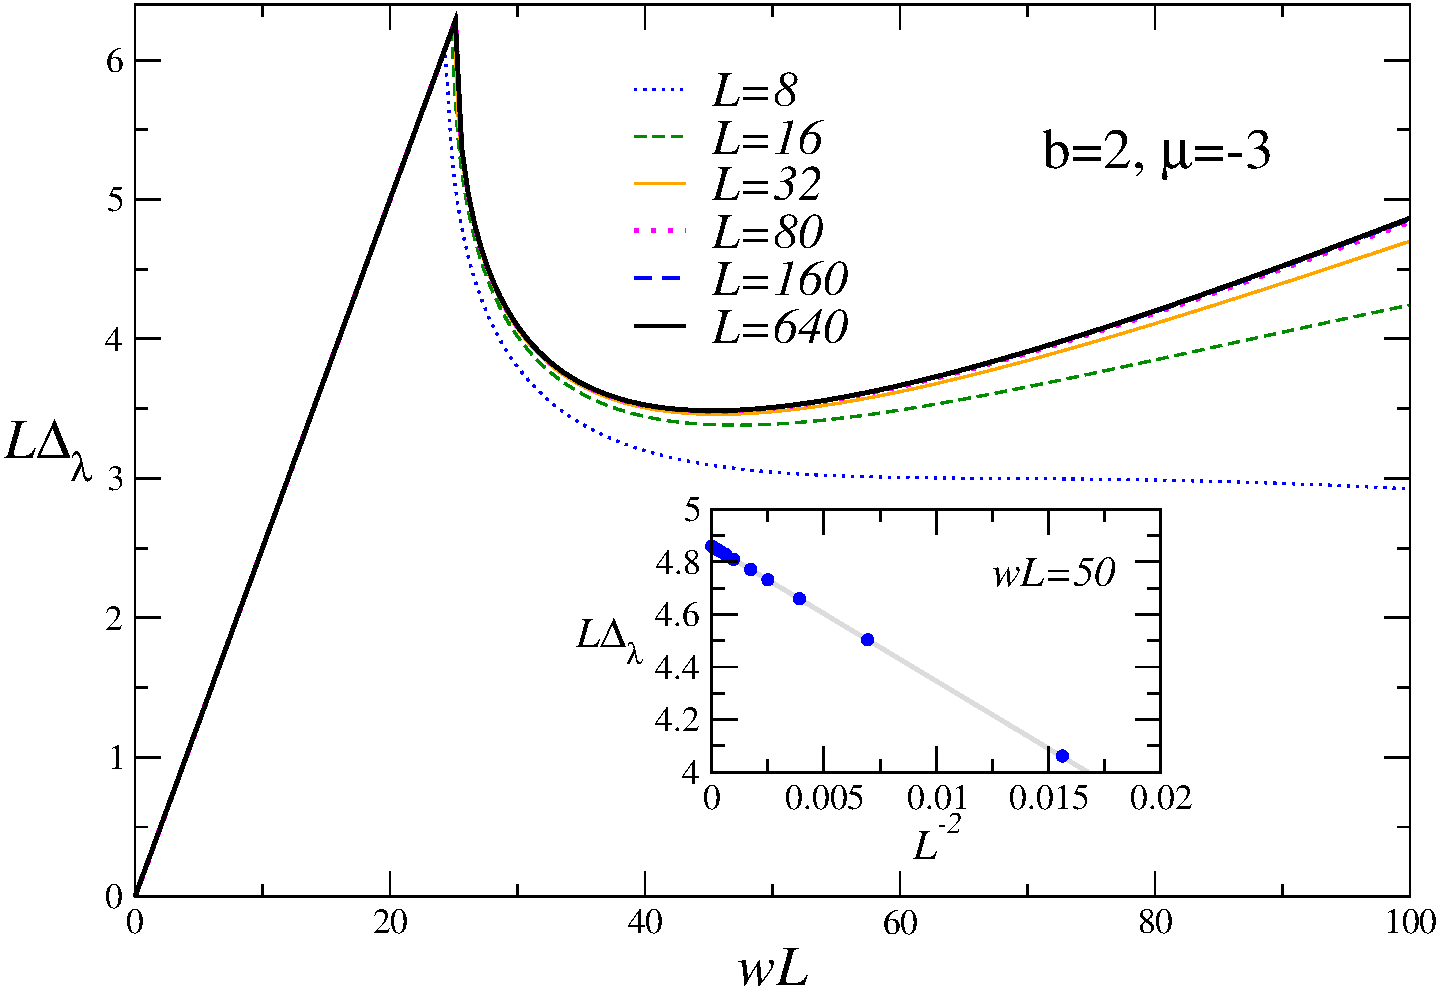
\includegraphics[width=6.4cm]{imm/scalingDeltaapbc.pdf}
    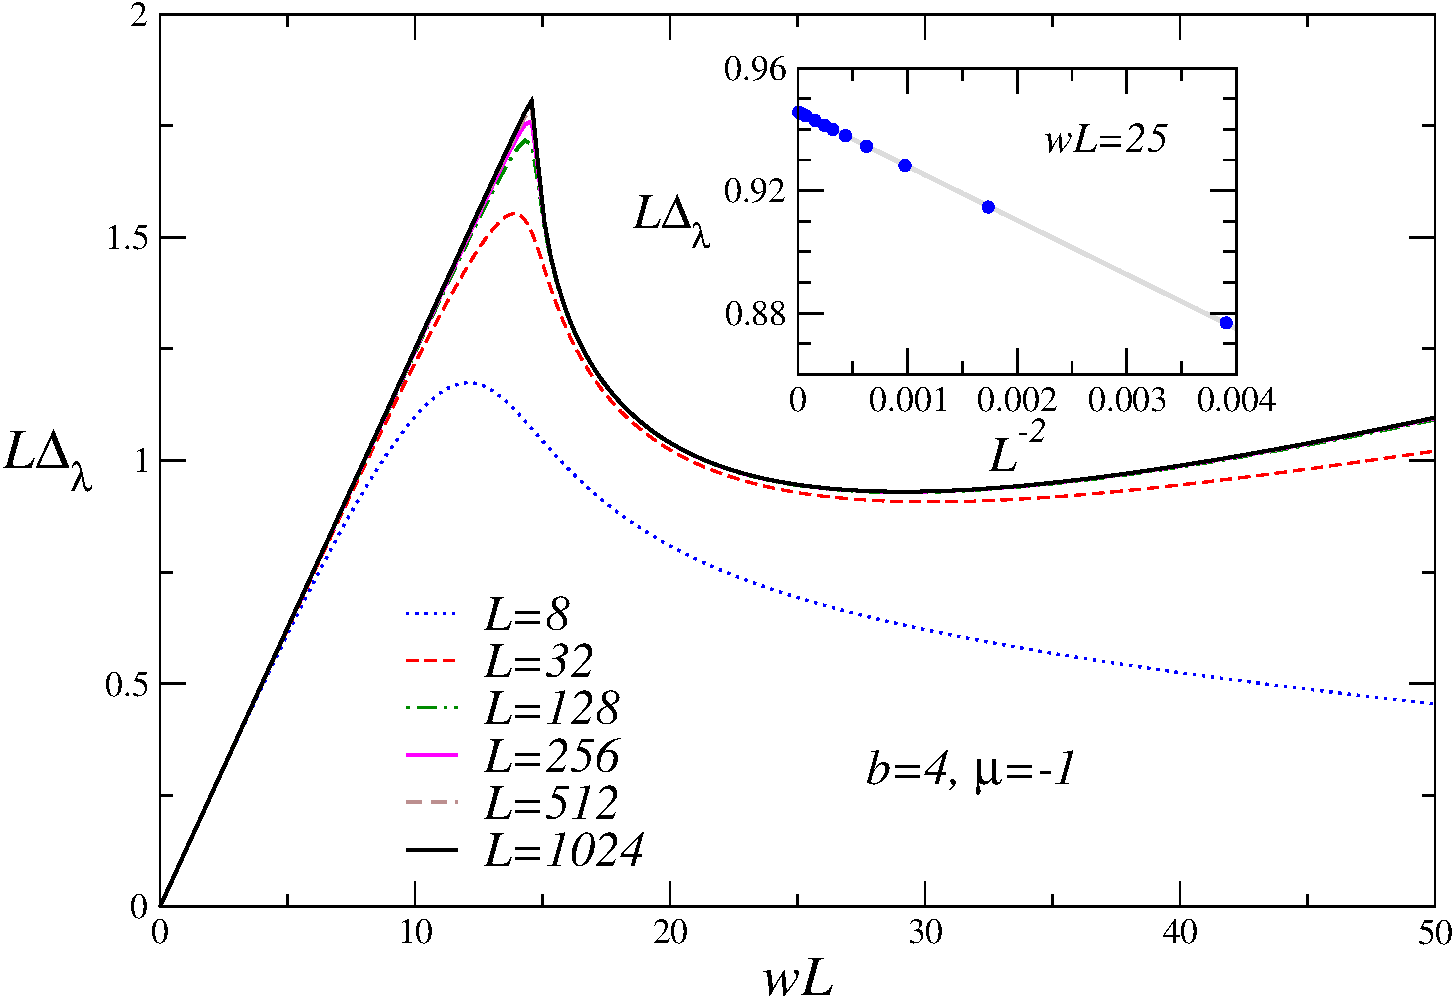
\includegraphics[width=6.4cm]{imm/scalingDelta4bmuminus1.pdf}
    \caption{Scaling of $L \Delta_\lambda$ versus $w L$ for different values of $b$ and $\mu$. On the top panel, we show results for $b=2$ and $\mu=-3$, while on the bottom panel, we fix $b=4$ and $\mu=-1$. The figures show an excellent data collapse in agreement with $L^{-2}$ scaling corrections. The straight lines in the insets are drawn to guide the eye.}
    \label{fig_scaling_delta_apbc}
\end{figure}



\subsubsection{Liouvillian gap at fixed $n$}
\label{sec_liouvillian_gap_fixed_n}

Now we start to study the behavior when we keep $n=L/b$ fixed. Since the number of the
external baths scales with the system size $L$, we will apply the third quantization 
technique, cited above.

The Fig.~\ref{fig_rescaleddelta_apbc_nfixed} shows that the gap scales as  
$\Delta_\lambda\sim L^{-3}$ at fixed $w$ in the regime $w>w_*$ ($w_\star$ is the maximum
point). This scaling is correlated also to the Eq.\eqref{eq_liouvillian_gap_largeL} and
simple matching arguments.\\



\begin{figure}[!t]
    \centering
    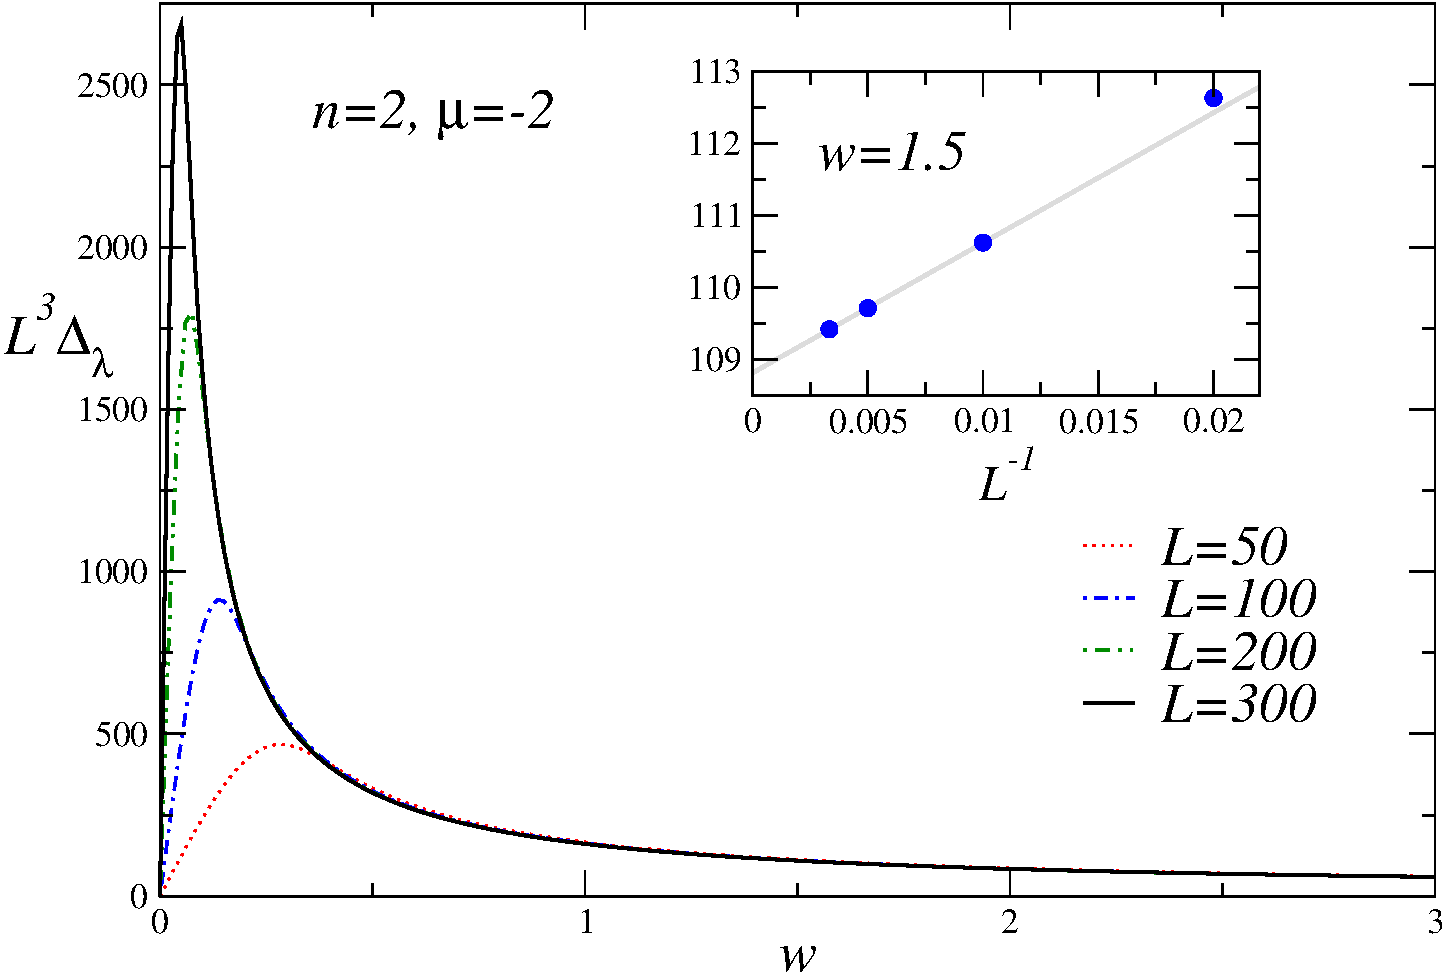
\includegraphics[width=8cm]{imm/delantipk0bl2L3Dw.pdf}
    \caption{Plot of the rescaled gap $L^3\Delta_\lambda$ in terms of $w$ for fixed $n=2$ and $\mu=-2$.  At fixed $w$, the gap shows a nice data collapse within $L^{-1}$ scaling corrections, as provided by the inset for the case $w=1.5$. The straight line is drawn to guide the eye.}
    \label{fig_rescaleddelta_apbc_nfixed}
\end{figure}

\begin{figure}[!b]
    \centering
    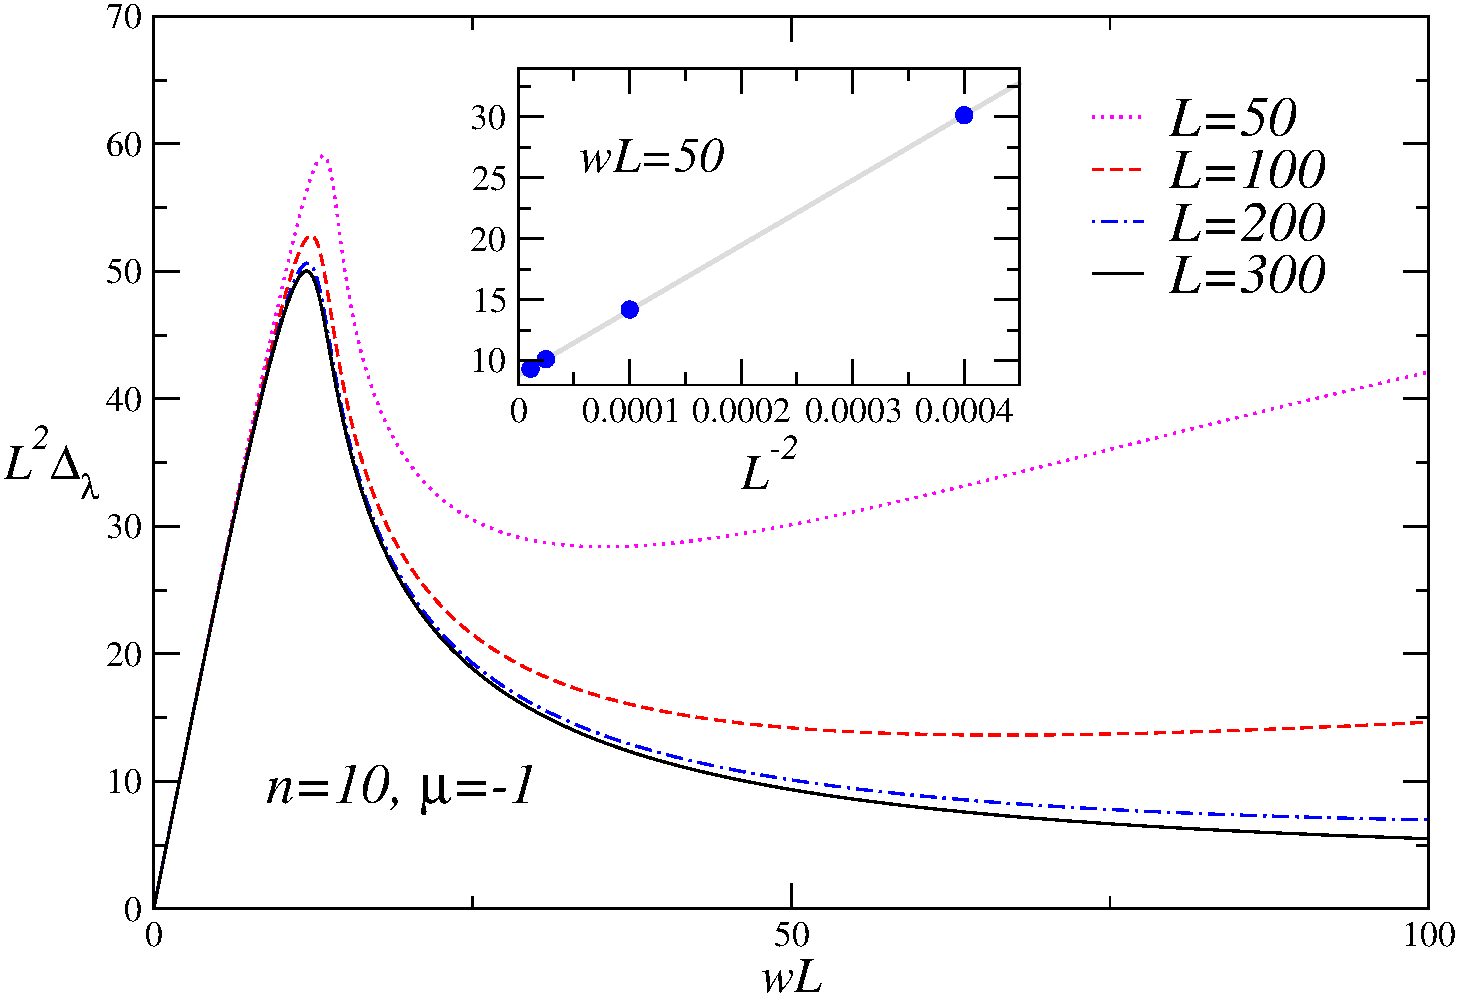
\includegraphics[width=8cm]{imm/scalingDeltanfixedmuminus1.pdf}
    \caption{The figure shows the Liouvillian gap $L^2\Delta_\lambda$ versus $w$ at fixed $n=10$ for $\mu=-1$. In the inset, scaling corrections at $wL=50$ are consistent with a decay $L^{-2}$. The straight line is drawn to guide the eye.}
    \label{fig_scalingDeltanfixed}
\end{figure}

Referring to Fig.~\ref{fig_rescaleddelta_apbc_nfixed}, when $w<w_*$ the gap does not show a uniform limit for $w\to0^+$ as the maximum of $L^3\Delta_\lambda$ grows without bounds with increasing $L$. We shed some light on this peculiar trend in Fig.~\ref{fig_scalingDeltanfixed}, considering the structure of the gap in the proximity of $w=0$ at fixed $n=10$ and $\mu=-1$. In fact, the plot supports the existence of a scaling regime for $L^2\Delta_\lambda$ when $w$ is properly rescaled as $w \sim 1/L$. Scaling corrections are also compatible with a decaying $L^{-2}$, as shown in the corresponding inset. We stress again that numerical results for different values of $\mu$ do not exhibit remarkable differences. We conclude that the different scaling regimes shown by the Liouvillian gap do not depend either on $\mu$ or the quantum phase related to the Kitaev model.


\subsection{Dynamic FSS Framework}


In this section, we study the time evolution of the Kitaev ring in the proximity of a CQT. To this end, we exploit a dynamic FSS framework and use RG arguments to describe the evolution of the critical correlations. Concerning the algorithms adopted, we speed up our simulations by moving to the momentum basis every time we maintain $b$ fixed. On the other hand, when $n$ is fixed, we just monitor the evolution of the two-point correlation functions by solving a closed system of differential equations. To evolve the density matrix $\rho$ in time, we use standard $4^{\text{th}}$-order Runge-Kutta techniques with typical integration time steps of $\Delta t=0.01$.

\subsubsection{The quench protocol and the monitored observables}
\label{sec_observables}

We now present the quench protocol considered to study the time evolution of the open quantum system under scrutiny at CQTs. We prepare the system in the ground state $\ket{\Omega}$ of Eq.~\eqref{kitaev2}. The starting chemical potential $\mu_i$ is always close to the critical value $\mu_c$, meaning that $\abs{\mu_i-\mu_c}\to0$ for $L\to\infty$. At a reference time $t=0$, the ring is driven out-of-equilibrium by suddenly coupling the system with the surrounding environment and eventually quenching the chemical potential to a different value $\mu_i\to\mu_f$. In such a case, the final $\mu_f$ should always be sufficiently close to the critical point. 

We monitor the time evolution of the Kitaev ring by considering two distinguished two-point correlation functions $C(x, y, t)$ and $P(x, y, t)$, defined as
\begin{align}
	C(x, y, t)&\equiv{\rm Tr}[\rho(t)(\hat{c}^\dagger_x\hat{c}_y+\hat{c}^\dagger_y\hat{c}_x)]\,,\\
	P(x, y, t)&\equiv{\rm Tr}[\rho(t)(\hat{c}^\dagger_x\hat{c}^\dagger_y+\hat{c}_y\hat{c}_x)]\,.
    \label{eq_def_two_point_functions_C_P}
\end{align}

%%===============================================================================

\subsection{Out-of-equilibrium FSS frameworks at CQTs with $b$ fixed}
\label{sec_Out-of-equilibrium FSS at CQT}

To describe the time evolution of the system under study at CQTs, we employ RG arguments and a dynamic FSS framework~\cite{C-1996-ScalingandRG, RV-2021-coherentanddissipativedynamicsreview}. The interplay between the unitary and dissipative dynamics of a Kitaev ring subject to complete bulk dissipation ($b=1$) has already been addressed in Ref.~\cite{NRV-2019-competingdissipativeandcoherent}. The results presented in this section extend the FSS reported in that work to all the cases with fixed $b>1$, and provide a complementing discussion on the role of $\Delta_\lambda$ in such a regime. Let us first review the main ideas leading to the FSS theory that we are going to discuss.

When we consider the time evolution of an open quantum system after a quench, analogous equations are more involved given the presence of a larger number of scaling quantities and relevant perturbations. First of all, we need to introduce a pre- and a post-quench scaling field $M_{i/f}=(\mu_{i/f}-\mu_c)L^{y_\mu}$ for $\mu$. In the second place, the time variable $t$ requires a scaling field as well. The most natural guess, which also turns out to be the correct one in most cases, is to rescale $t$ with $L$ on the basis of the dynamic critical exponent $z$. We then introduce the quantity $\Theta$ defined as
\begin{equation}
    \Theta = t L^{-z}\,, \quad z=1\,,
    \label{eq_def_Theta_scaling}
\end{equation}
which is maintained constant in the FSS limit.
Since the number of particle-decay jump operators increases as $L$, we also need to soften the coupling $w$ to observe an interplay between the critical and dissipative modes. We note that the parameter $w$ plays the role of
a decay rate, namely, it is an inverse relaxation time~\cite{NRV-2019-competingdissipativeandcoherent, BP-openquantumsystembook}.
In our work hypothesis, we then suppose that $w$ should be rescaled with $L^{-z}$ to observe universal FSS relations. We introduce the scaling field $\gamma_b$ as
\begin{equation}
    \gamma_b=\frac{wL^{z}}{b}\,,\quad z=1.
    \label{def_gamma_scaling}
\end{equation}
Naturally, the prefactor $b^{-1}$ appearing in $\gamma_b$ is just a matter of convention if one restricts the analysis to just one value of $b$. However, the comparison between different values of $b$ in the FSS limit may add new valuable insights to our analyses. To compare the dissipative processes of different rings on the same footing, we assume that the effective coupling strength is $w/b$. This choice is the most natural one considering the Kitaev ring in momentum space. 

\begin{figure}
    \centering
    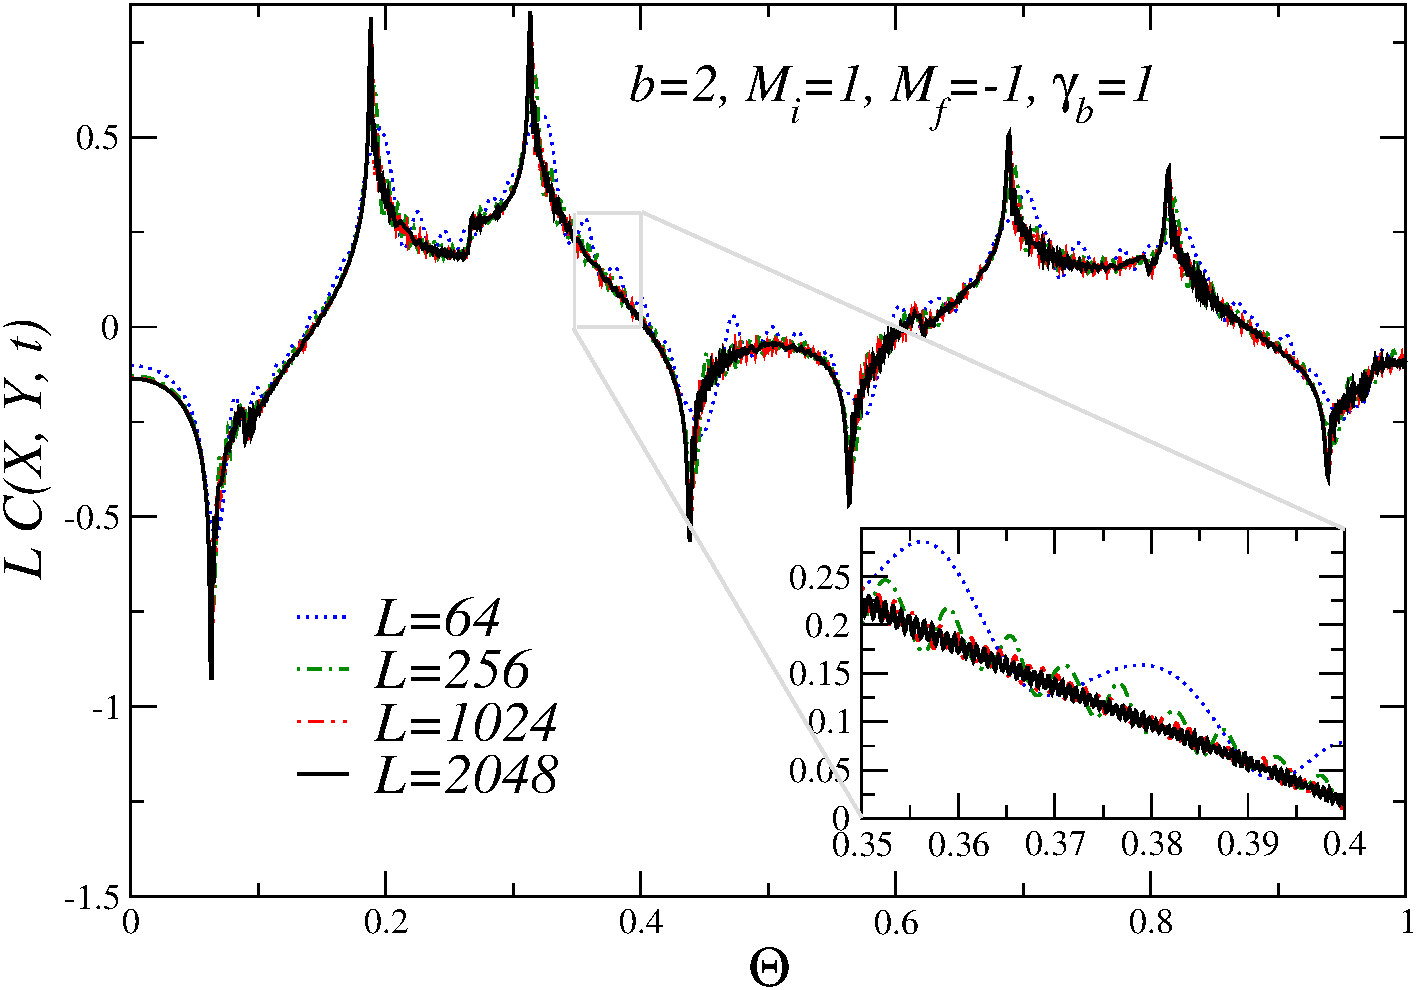
\includegraphics[width=7cm]{imm/Cscaling2b.pdf}
    \caption{Scaling of the two-point function $L C(X, Y)$ in terms of the scaling variable $\Theta$ for fixed $b=2$, $M_i=1$ and $\gamma_b=1$. We consider $(Y-X)/L=1/4$ and fix $x=1$, using translation invariance. In the inset, we show a zoom of the region $\Theta\in[0.35, 0.4]$. Our data clearly support the FSS laws exhibited in Eq.\eqref{eq_scaling_C}.}
    \label{fig_Cscaling2b}
\end{figure}

The universal scaling relations satisfied by the two-point functions $C$ and $P$ in Eq.~\eqref{eq_def_two_point_functions_C_P} follows
\begin{align}
    C(x, y, t) &\approx L^{-2y_c}\mathcal{C}(M_i, M_f, \{X_i\}, \Theta, \gamma_b)    \label{eq_scaling_C}\\
    P(x, y, t) &\approx L^{-2y_c}\mathcal{P}(M_i, M_f, \{X_i\}, \Theta, \gamma_b)\,,
    \label{eq_scaling_P}
\end{align}
where $y_c=1/2$ is the scaling dimension of both $\hat{c}$ and $\hat{c}^\dagger$. 
In Fig.~\ref{fig_Cscaling2b} we show the scaling of $LC(X, Y, t)$ in terms of the scaling quantity $\Theta$ for $b=2$, $M_i=1$, $M_f=-1$, and $\gamma_b=1$. The panel definitely supports the FSS laws exhibited in Eq.~\eqref{eq_scaling_C}. In the inset, we show that the amplitude of the oscillations reduces at fixed $\Theta$ and increasing $L$, roughly as $\sim L^{-1/2}$. We have checked that Eq.~\eqref{eq_scaling_P} holds also for the scaling of the RG invariant quantity $LP(X, Y, t)$ (not shown).  
\subsection{Out-of-equilibrium FSS framework at CQTs with $n$ fixed}
\label{sec_out-of-equilibrium FSS fixed n}

\begin{figure}
    \centering
    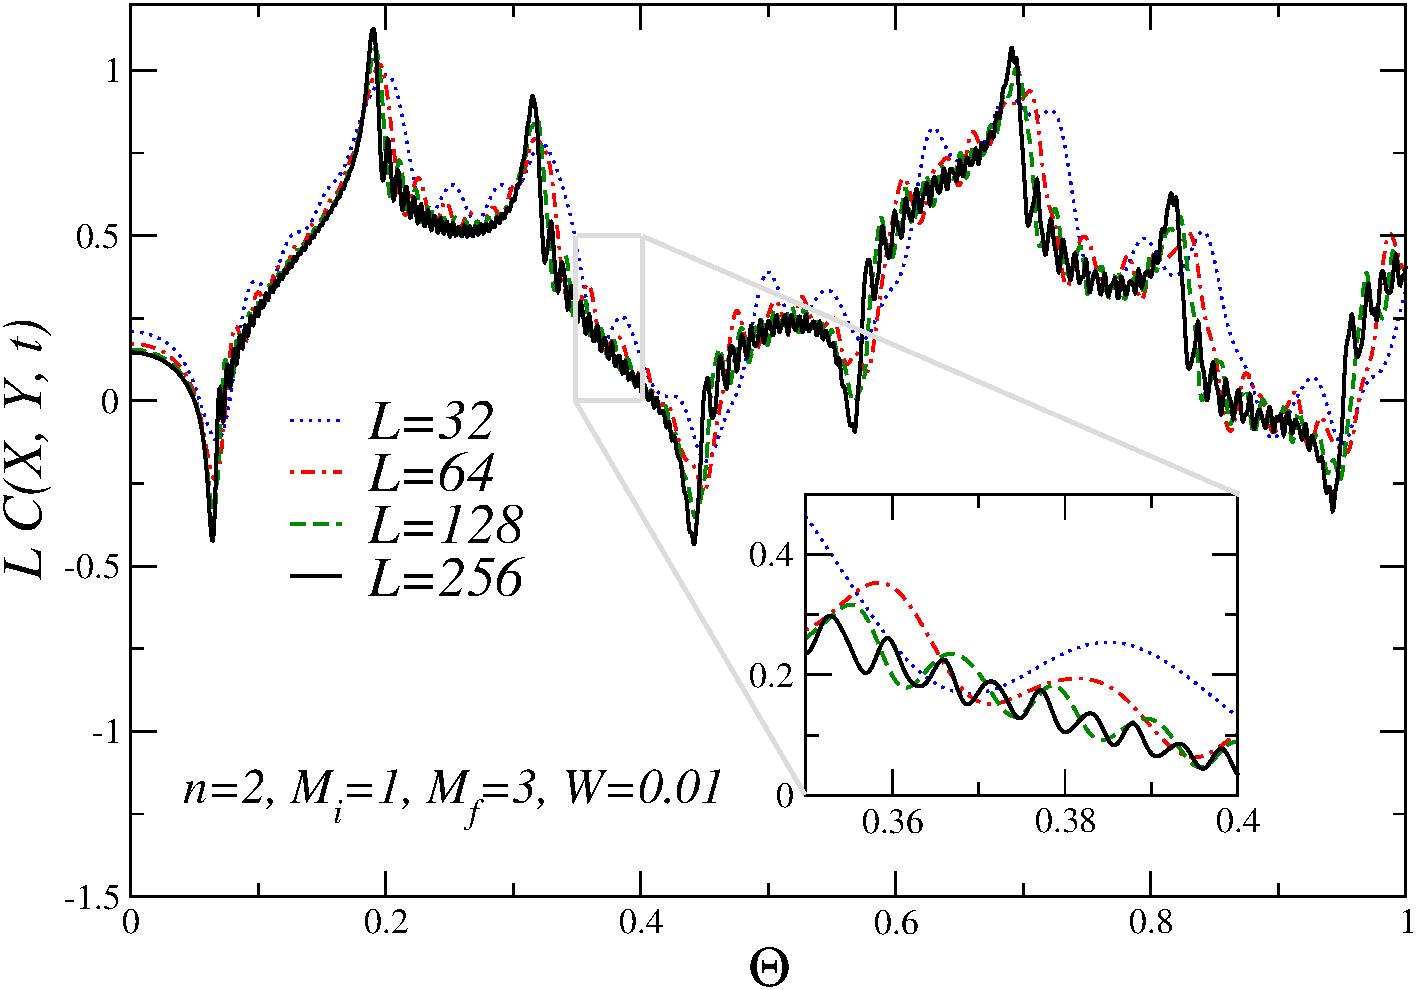
\includegraphics[width=7cm]{imm/fssnfixed2n.pdf}
    \caption{Scaling of the rescaled two-point correlation function $L C(X, Y)$ in terms of $\Theta$ for fixed of $n=2, M_i=1, M_f=3$, and $W=0.01$. We consider $Y-X=L/4$, exploiting translation invariance, and fix the first site to $x=1$ in conjunction with a dissipator. We zoom in on the domain $\Theta\in[0.35, 0.4]$ to emphasize the convergence of different curves with increasing lattice size $L$.}
    \label{fig_fss_2n_fixed}
\end{figure}

In this section, we derive a dynamic FSS framework at CQTs to study the time evolution of Eq.~\eqref{eqlindblad} when the number of the dissipators $n$ is fixed. Most of the scaling relations of the last section are still valid at fixed $n$ with straightforward generalizations. In particular, we just replace the coupling $w$ in our relations, which now represents a decay rate per unit space since $b\sim L$. As a working hypothesis, we expect the scaling field $W$, defined as
\begin{equation}
    W = w L^{z-1}\,, \quad z=1\,,
    \label{eq_def_scaling_variable_W}
\end{equation}
to be a reasonable scaling quantity in the FSS limit. 
For instance, the critical correlations satisfy scaling relations similar to the ones reported in Eq.~\eqref{eq_scaling_C}
\begin{align}
    C(x, y, t)\approx& L^{-2y_c}\mathcal{C}(M_i, M_f, \{X_i\}, \Theta, W)\\
    P(x, y, t)\approx& L^{-2y_c}\mathcal{P}
    (M_i, M_f, \{X_i\}, \Theta, W)\,.
    \label{eq_def_CP_scaling_n_fixed}
\end{align}

We verify our hypotheses in Fig.~\ref{fig_fss_2n_fixed}, showing the scaling curve for $L C(X, Y, t)$ versus the scaling variable $\Theta$ with constant $n=2, M_i=1, M_f=3, W=0.01$. We obtain a nice data collapse considering lattice sizes up to $L=256$. The oscillation amplitudes shrink with increasing $L$, converging to a universal asymptotic curve $\mathcal{C}$. The validity of Eq.~\eqref{eq_def_CP_scaling_n_fixed} has been checked also by inspecting the time evolution of $L P(X, Y, t)$ (not shown).



\begin{comment}
    
\section{Summary}

When we keep $b$ fixed, the gap $\Delta_\lambda$ is always finite and depends linearly on the dissipation strength $w$. Nonetheless, two different regimes emerge for systems of finite size. In the small $w$ region, the gap is given by $\Delta_\lambda=w/(2b)$, whereas, at large $w$ and sufficiently large $b$, it behaves as $\Delta_\lambda=w C_\mu/b^3$. The last equation always controls the gap in the large-size limit and is our starting point to deduce the scaling of such a quantity when $b\propto L$. It is worth mentioning that we also put forward a scaling regime for $L\Delta_\lambda$ as a function of $wL$, which ties together the two different regimes outlined in a smooth manner. On the other hand, when we keep the number of dissipators $n$ fixed, the gap vanishes as $\sim L^{-3}$ at large $L$. Addressing the structure of the gap at small $w$, we find a scaling regime for $L^2\Delta_\lambda$ in terms of $wL$, which is closely related to the presence of a non-uniform convergence of $L^3\Delta_\lambda$ in the limit $w\to0^+$.\\

We develop a dynamic FSS regime at CQTs to describe the time evolution of the Kitaev model under investigation. At fixed $b$, our results extend the FSS theory of Ref.~\cite{NRV-2019-competingdissipativeandcoherent} to the cases with $b>1$. As a working hypothesis, we suppose that the scaling variable associated with the relevant coupling $w$ is $\gamma_b=wL^{z}/b$. Our numerical results for the two-point correlation functions fully support this ansatz. When the number of dissipators $n$ is fixed, the FSS theory outlined at fixed $b$ generalizes straightforwardly after replacing $\gamma_b$ with $W=wL^{z-1}$. 

%In the last section, we analyze the interplay between the Liouvillian gap $\Delta_\lambda$ and the gap related to the Kitaev ring $\Delta$ in the FSS limit. In particular, we take into account the short- and long-time regimes, focusing on how they join together in the FSS limit. When $b$ is fixed, we observe that the link between the two regimes is smooth, whereas, at fixed $n$, the two regions can be easily distinguished given the presence of different power-law scalings for the gaps $\Delta$ and $\Delta_\lambda$. 
\end{comment}




\section{Thermal-bath effects in quantum quenches}

%\subsection{Kitaev fermionic wires and thermal baths}
\label{modbath}

\subsection{The fermionic Kitaev chain}
\label{kitaevmod}

We consider fermionic Kitaev wires of $L$ sites with open boundary
conditions, whose quantum unitary dynamics is driven by the
Hamiltonian~\cite{Kitaev-01}
\begin{equation}
  \hat H_{\rm K} = - J \sum_{x=1}^{L-1} \big( \hat c_x^\dagger \hat
  c_{x+1}^{\phantom\dagger} +
  \hat c_x^\dagger \hat c_{x+1}^\dagger+{\rm h.c.}
  \big) - \mu \sum_{x=1}^L \hat n_x ,
  \label{kitaev2}
\end{equation}
where $\hat c_x$ is the fermionic annihilation operator associated
with the site $x$ of the chain, $\hat n_x\equiv \hat
c_x^\dagger \hat c_x^{\phantom\dagger}$ is the particle density
operator.  In the following we assume $J$ as the energy scale, thus we
set $J=1$.

The Hamiltonian~\eqref{kitaev2} can be mapped into a quantum Ising
chain, by means of the Jordan-Wigner transformation, see, e.g.,
Ref.~\cite{Sachdev-book}.  The corresponding spin model is the
quantum Ising chain with open boundary conditions, i.e.
\begin{equation}
  \hat H_{\rm Is} = -\sum_{x=1}^{L-1} \hat \sigma^{(1)}_x \hat
  \sigma^{(1)}_{x+1} - g\, \sum_{x=1}^L \hat \sigma^{(3)}_x,
  \label{isham}
\end{equation}
$\hat \sigma^{(k)}_x$ being the Pauli matrices and $g=-\mu/2$.  In the
following we prefer to stick with the Kitaev quantum wire, because the
thermal baths and observables that we consider are best defined within
the fermionic model. However, the general scaling scenarios that will
emerge apply to both models.

The Kitaev model undergoes a CQT at $\mu=\mu_c = -2$ (corresponding to
$g=g_c=1$ in the quantum Ising chain), between a disordered quantum
phase for $\mu<\mu_c$ (corresponding to $g>1$) and an ordered quantum
phase for $|\mu|<|\mu_c|$ (corresponding to $|g|<1$). Thus, we define
\begin{equation}
  w = \mu - \mu_c = \mu + 2,
  \label{wdef}
\end{equation}
so that one can easily see the correspondence between the Kitaev
Hamiltonian (\ref{kitaev2}) and the generic one reported in
Eq.~(\ref{qudef}), i.e. $\hat{H}_c$ corresponds to the Hamiltonian
(\ref{kitaev2}) for $\mu=\mu_c$, and $\hat{H}_p=-\sum_{x=1}^L \hat
n_x$.  The continuous transition at $w=w_c$ belongs to the
two-dimensional Ising universality class~\cite{Sachdev-book,RV-21},
characterized by the length-scale critical exponent $\nu=1$, related
to the RG dimension $y_w = 1/\nu=1$ of the Hamiltonian parameter
$w$. This implies that, approaching the critical point, the length
scale $\xi$ of the critical quantum fluctuations diverges as $\xi \sim
|w|^{-\nu}$. The dynamic exponent $z=1$ associated with the unitary
quantum dynamics can be obtained from the power law
$\Delta\sim\xi^{-z}$ of the vanishing gap with increasing $\xi$.
Moreover, the RG dimension of the fermionic operators $\hat c_j$ and
$\hat c^\dagger_j$ at the CQT is $y_c = 1/2$, and that of the particle
density operator $\hat n_x$ is $y_n = 1$~\cite{Sachdev-book,RV-21}.


\subsection{Modelization of the thermal bath}
\label{thebath}

In our study we consider a modelization of interaction with a thermal
bath within the Lindblad master equation (\ref{Lindblad}), whose
asymptotic large-time behavior leads to a Gibbs density matrix at a
given finite temperature $T$. In particular, we consider the proposal
developed in Ref.~\cite{DR-21} which applies to quantum models
described by quadratic Hamiltonians, such as that of the fermionic
Kitaev wires. This provides a relatively simple modelization of a
thermal bath leading to thermalization in the large-time limit of the
corresponding Lindblad master equation for the density matrix of the
system.

The Kitaev Hamiltonian (\ref{kitaev2}) with open boundary conditions
can be diagonalized in the Nambu field space by a Bogoliubov
transformation, see e.g. Refs.~\cite{Pfeuty-70,BR-book,DR-21}, so that
we can rewrite it as
\begin{equation}
\hat{H}_{\rm K}=\sum_{k=1}^L\,\omega_k \,\hat b^\dagger_k\, \hat b_k,
  \label{Hdiag}
\end{equation}
where $\omega_k$ are values of the spectrum of the Bogoliubov
eigenoperators $\hat b_k$ (we are neglecting an irrelevant constant
term). Note that both $\omega_k$ and $\hat b_k$ depend on the
Hamiltonian parameter $\mu$.  The relation between the fermionic
operators $\hat{c}_x$ and the Bogoliubov eigenoperators $\hat{b}_k$
can be generally written as~\cite{Pfeuty-70,BR-book,DR-21}
\begin{equation}
  \label{transBogol}
  \hat c_x = \sum_{k=1}^L A_{xk} \,\hat{b}_k + B_{xk}
  \,\hat{b}_k^\dagger,
\end{equation}
where $A$ and $B$ are appropriate $L\times L$ matrices depending on
$\mu$.  Following Refs.~\cite{DR-21,PCR-22}, we write the dissipator
$\mathbb{D}_T[\rho]$ in the Lindblad master equation (\ref{Lindblad})
in terms of the Bogoliubov eigenoperators as
\begin{eqnarray}
  \mathbb{D}_T[\rho] &=&
\sum_k [1-f(\omega_k,T)]
\left( 2 \,\hat{b}_k\,\rho\,\hat{b}_k^\dagger - 
\{\hat{b}_k^\dagger\hat{b}_k,\rho\}\right)  \nonumber\\
&+&
\sum_k f(\omega_k,T)
\left( 2 \,\hat{b}_k^\dagger\,\rho\,\hat{b}_k - 
\{\hat{b}_k\hat{b}_k^\dagger,\rho\}\right), \label{Dtrho}
\end{eqnarray}
where
\begin{equation}
  f(\omega_k,T) = \left( 1 + e^{\omega_k/T}\right)^{-1}.
  \label{fomt}
\end{equation}
When using this homogeneous dissipator term, the Lindblad master
equation (\ref{Lindblad}) ensures the asymptotic large-time
thermalization~\cite{DR-21}. Therefore,
\begin{eqnarray}
  &&\lim_{t\to\infty} \rho(t)  = \rho_t(w,T), \label{asyrho}\\
&&\rho_t(w,T) = \sum_n e^{-E_n(w)/T}|\Phi_n, w\rangle \langle \Phi_n, w|,
 \qquad \label{termrho}
\end{eqnarray}
where $\rho_t(w,T)$ is the density matrix representing the thermal
state, $E_n(w)$ and $|\Phi_n, w\rangle$ are the eigenvalues and
eigenstates of $\hat{H}(w)$.  The asymptotic approach to the thermal
distribution is controlled by the decay-rate parameter
$\gamma$~\cite{DR-21}. Indeed the Liouvillian gap $\Delta_{\cal L}$
that controls the exponential approach to the asymptotic stationary
state of the Lindblad equation is proportional to the decay rate
$\gamma$, i.e.
\begin{equation}
  \Delta_{\cal L}\sim \gamma.
  \label{deltal}
  \end{equation}

The above modelization of thermal baths provides a useful theoretical
laboratory to investigate issues related to the out-of-equilibrium
dynamics in the presence of thermal baths. Its derivation has
been thoroughly discussed in Ref.~\cite{DR-21}. We also mention that it
has been employed in Refs.~\cite{PCR-22,BD-23}.  Some details of the
computations using the Lindblad master equation (\ref{Lindblad}) with
the dissipator (\ref{Dtrho}) are reported in the appendix.


\subsection{Quantum-quench protocols}
\label{proto}

As already anticipated in Sec.~\ref{intro}, we consider two protocols,
differing for the absence or presence of the contact with the thermal
bath during the quantum evolution after quenching, giving respectively
rise to unitary or dissipative dynamics after quenching. We call them
{\em unitary} and {\em dissipative} QQ protocols, respectively.

\begin{itemize}

\item {\em Unitary} QQ protocol: In this simplest QQ protocol the role
  of the thermal bath is limited to that of preparing the initial
  Gibbs state $\rho_t(w_i,T)$ at $t=0$, reported in
  Eq.~(\ref{rhoi}). This can be obtained by keeping the thermal bath
  in contact with the system for a sufficiently long time $t_{\rm th}$, i.e
  $t_{\rm th}\gg \gamma^{-1}$. Then at $t=0$ the Hamiltonian parameter is
  instantaneously quenched from $w_i<0$ to $w\ge 0$ and the thermal
  bath is removed, so that the subsequent time evolution is that of a
  closed fermionic wire, i.e.  it is unitary and only driven by the
  Hamiltonian of the system, cf. Eq.~(\ref{firstprot}).

\item {\em Dissipative} QQ protocol: The quantum evolution starts from
  the same initial Gibbs state $\rho_t(w_i,T)$, but the thermal bath
  is maintained in contact with the system after the QQ from $w_i<0$
  to $w\ge 0$, at $t=0$.  Therefore, the quantum evolution for $t>0$
  is driven by the Lindblad master equation (\ref{Lindblad}) with the
  dissipator term (\ref{Dtrho}). Note that this dynamic protocol
  entails a further time scale $\tau = \gamma^{-1}$, characterizing
  the asymptotic exponential approach to the large-time stationary
  Gibbs state associated with the Hamiltonian $\hat{H}(w)$ and
  temperature $T$.

\end{itemize}


\subsection{Observables monitoring the time evolution}
\label{obs}


To characterize the dynamic properties of the quantum evolution after
the QQ at $t=0$, we consider the subtracted particle-density average
\begin{eqnarray}
n_s(t,L) = {1\over L} {\rm Tr} \left[ \rho(t) \sum_{x=1}^L \hat{n}_x \right]
- n_c(L),
 \label{ddef}
\end{eqnarray}
 where $n_c(L)$ is the ground-state energy density of the Kitaev wire
 of size $L$ at the critical point $w_c=0$ (in the infinite-size limit
 $n_c= 1/2 - 1/\pi$~\cite{Pfeuty-70}). Note that the particle density
 operator $\hat{n}_x$ and the transverse spin component
 $\hat\sigma_x^{(3)}$ of the quantum Ising chain (\ref{isham}) are
 trivially related, indeed $\hat{\sigma}_x^{(3)} = 2 \hat{n}_x$.  In
 the definition of $n_s$, the subtraction of $n_c(L)$ simplifies the
 scaling behavior of $n_s(t,L)$ within the critical regime, cancelling
 the leading analytical behavior~\cite{CPV-14,RV-21}. To monitor the
 spatial correlations, we also consider
\begin{eqnarray}
P(x,y,t) & \!\! = \!\! & {\rm Tr}[\rho(t)\,(\hat c_x^\dagger 
\hat c_{y}^\dagger +
    \hat c_{y} \hat c_{x})],\label{ptf}\\ 
C(x,y,t) & \!\! = \!\! & {\rm Tr}[\rho(t)\, (\hat c_x^\dagger \hat c_{y} 
+ \hat
    c_{y}^\dagger \hat c_{x})].\label{gtf} 
\end{eqnarray}

Some details on the computation of the above quantities during the
time evolution of the QQ protocols are reported in the appendix.


\subsection{Out-of-equilibrium scaling}
\label{scabeh}

We now discuss the out-of-equilibrium behaviors arising from the QQ
protocols outlined in Sec.~\ref{proto}.  We show that they develop
OFSS behaviors where the effects of the thermal baths are taken into
account by appropriate extensions of the out-of-equilibrium
zero-temperature scaling laws describing soft QQs in
closed systems within their critical regime, already put foward by
earlier works~\cite{PRV-18,RV-21}.

\begin{figure}[!htb]
\centering
  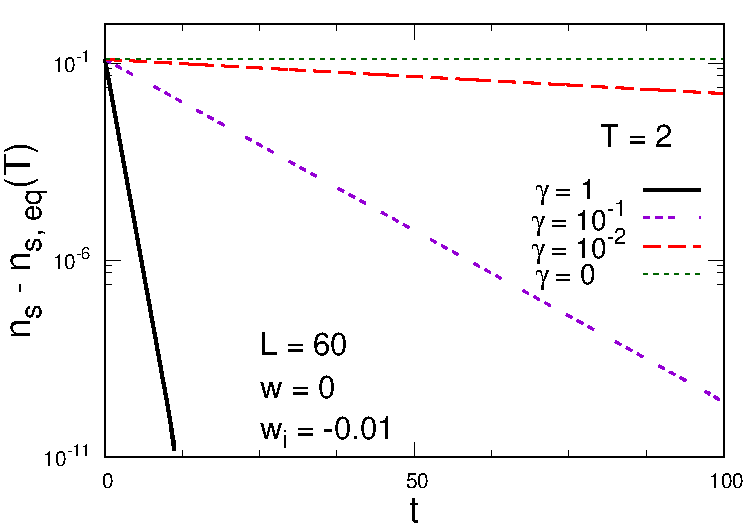
\includegraphics[width=0.6\columnwidth]{imm/NT2l60diffglog.pdf}
  \caption{The quantum evolution of the subtracted particle density
    $n_s(t)$, cf. Eq.~(\ref{ddef}), for the dissipative QQ protocol
    entailing a dissipative dynamics after the QQ at $t=0$ of the
    Hamiltonian parameter $w$, describing the persistent interaction
    with the thermal bath, cf.  Eqs.~(\ref{Lindblad}) and
    (\ref{Dtrho}).  These curves refer to a system of size $L=60$,
    temperature $T=2$ of the thermal bath, quenching from $w_i=-0.01$
    to $w=0$, and various values of the decay rate $\gamma$ (the case
    $\gamma=0$ corresponds to the evolution of the close system).  We
    plot the difference $n_s(t,L,T) - n_{s,{\rm eq}}(L,T)$ which is
    expected to vanish in the large-time limit.  In this figure and in
    the following ones, the unity that we use are such that
    $\hslash=1$, $k_B=1$, and $J=1$.}
  \label{plainns}
\end{figure}



The OFSS behaviors that we put forward for QQ protocols considered are
verified by numerical computations for the fermionic Kitaev wire up to
relatively large sizes. See the appendix for details on such
calculations.

As a preliminary example of out-of-equilibriun QQ
behaviors that we want to address, in Fig.~\ref{plainns} we show some
results for the quantum evolution of the subtracted particle density
(\ref{ddef}) along the dissipative protocol outlined in
Sec.~\ref{proto}, after quenching a fermionic Kitaev wire of size
$L=60$, from $w_i=-0.01$ to $w=0$, in the presence of a thermal bath
at a temperature $T=2$, and various values of the decay rate $\gamma$.
The quantum evolution turns out to have a significant dependence on
the decay-rate parameter $\gamma$ that characterized the interactions
between the system and the thermal bath. Indeed, the curves of the
substracted particle density appear to approach its equilibrium value
$n_{s,{\rm eq}}(w=0,T=2)\approx 0.0004601...$ (while at $t=0$ we have
$n_{s,{\rm eq}}(w=w_i,T=2) \approx 0.126598...$), faster and faster
with increasing $\gamma$, actually exponentially as $\exp(-t/\tau)$
with $\tau\sim\gamma^{-1}$, conferming the role of decay rate of the
parameter $\gamma$ within the Lindblad master equation,
cf. Eq.~(\ref{deltal}). Analogous results are obtained for other
observables, such as fermionic correlation functions defined in
Sec.~\ref{obs}. In the following we put forward an out-of-equilibrium
scaling theory for these out-of-equilibrium phenomena within the
quantum critical regime.




\subsubsection{Zero-temperature scaling in quantum quenches}
\label{zeroT}

We now provide a brief summary of the out-of-equilibrium scaling
theory for close systems, describing QQ protocols within the critical
regime~\cite{PRV-18,RV-21}. The initial state is the ground state
associated with an initial value $w_i<0$, and, after the instantaneous
quench at $t=0$ from $w_i$ to $w$, the quantum evolution is driven by
the Schr\"odinger equation.

Out-of-equilibrium scaling laws can be obtained by extending those
valid at equilibrium, allowing for a time dependence essentially
controlled by the time scaling variable $\Theta \sim t\,\Delta$, which
is obtained by assuming that the relevant time scale of the critical
modes is proportional to the inverse energy difference $\Delta$ of the
lowest states. We refer to Ref.~\cite{RV-21} for a through
presentation of the scaling arguments leading to the asymptotic OFSS
behaviors.

Let us consider the out-of-equilibrium evolution (after quenching) of
generic observables, such as the expectation value $O$ at time $t$ of
a local operator $\hat{O}({\bm x})$ and its fixed-time correlations
$G_O=\langle \hat{O}({\bm x}) \hat{O}({\bm y})\rangle$. The general
working hypothesis underlying out-of-equilibrium FSS frameworks is
that the expectation value of $\hat{O}({\bm x})$ and its correlation
functions obey asymptotic homogeneous scaling laws~\cite{RV-21}, such
as
\begin{eqnarray}
O(t, {\bm x}, L, w_i, w) \approx  b^{-y_o} {\cal O}(t/b^z,
{\bm x}/b, L/b, b^{y_w} w_i, b^{y_w} w),\quad
    \label{Oscaquefss0}
\end{eqnarray}
  where $b$ is an arbitrary (large) length scale, $y_o$ is the RG
  dimension of the local operator $\hat{O}_{\bm x}$ and the RG
  exponents $y_w$ and $z$ are determined by the universality class of
  the CQT (they are the RG dimensions of the Hamiltonian parameter $w$
  and the temperature $T$, respectively). Thus both the initial and
  final values of $w$, i.e.  $w_i$ and $w$, take the same RG exponent
  $y_w$, being coupled to the RG perturbation ${\hat H}_p$ within the
  Hamiltonian. Note that we do not assume translation invariance,
  which is generally broken by the presence of boundaries, such as
  those arising from open boundary conditions.
  
 
OFSS can be straightforwardly derived by fixing $b=L$ in the above
homogenous scaling law. Then, we expect the OFSS of the expectation
value $O$ of a generic local operator $\hat{O}_{\bm x}$, of its
spatial average $\hat{O}_a =L^{-d}\sum_{\bm x}\hat{O}_{\bm x}$, and
its two-point correlation function $G_O$, develop the asymptotic OFSS
behavior~\cite{PRV-18,RV-21}
\begin{eqnarray}
  && O(t, {\bm x}, L, w_i, w) \, \approx \, L^{-y_o} \,
  {\cal O}(\Theta, {\bm X}, \Phi_i, \Phi),
\nonumber\\
  && O_a(t, L, w_i, w) \, \approx \, L^{-y_o} \, {\cal O}_a(\Theta,
\Phi_i, \Phi),   \label{Oscaquefss}\\
  && G_{O}(t, {\bm x}_1, {\bm x}_2, L,
  w_i, w) \, \approx \, L^{-2y_o} \, {\cal G}_{O}(\Theta, {\bm X}_1,
  {\bm X}_2, \Phi_i, \Phi), \nonumber
\end{eqnarray}
where the scaling variables appearing in the scaling functions ${\cal
  O}$, ${\cal O}_a$, and ${\cal G}_O$ are defined as
\begin{equation}
  \Theta\equiv\frac{t}{L^z},\;\; {\bm X}_i \equiv \frac{{\bm x}_i}{L},\;\;
  \Phi_{i} \equiv
L^{y_w} \, w_i , \;\; \Phi \equiv L^{y_w} \,w.
  \label{scalvarque}
\end{equation}
The OFSS limit is obtained in the large-$L$ and large-$t$ limit
keeping the above scaling variables fixed. These conditions ensure
that the system remains within the universal critical regime during
the quantum evolution.  Note that in the scaling law
(\ref{scalvarque}) the dynamic features are essentially encoded in the
time dependence of the scaling variable $\Theta\sim t\,\Delta$.  The
other features, in particular when $w_i=w$, are analogous to those
arising from equilibrium FSS at CQTs~\cite{CPV-14,RV-21}, where the
argument $\Phi=L^{y_w} w$ of the scaling functions is controlled by
the RG dimension $y_w$ of the relevant parameters $w$ at the RG fixed
point associated with the CQT.


The above OFSS equations can be straightforwardly applied to the
observables defined in Sec.~\ref{obs}, after a quench from $w_i$ to
$w$ at $t=0$, keeping into account that the RG dimension of the
subtracted particle density is $y_n = 1$, and that of the fermionic
operator $\hat c_x$ is $y_c=1/2$.  Note that the dominant analytical
contributions to the particle density~\cite{CPV-14,RV-21} coming from
the analytical background are canceled in the difference $n_s$ defined
in Eq.~(\ref{ddef}), whose leading asymptotic behavior arises from the
quantum critical modes, therefore it is analogous to that of $O_a$ in
Eq.~(\ref{Oscaquefss}), with $y_o=y_n$.  Analogously one can apply the
OFSS in Eq.~(\ref{Oscaquefss}) to observables and correlation
functions constructed with the spin operators of the quantum spin
chain (\ref{isham}).  The OFSS functions are expected to be universal
with respect to the microscopic details of the model, apart from
nonuniversal multiplicative rescaling and normalizations of its
arguments.  Within isolated fermionc Kitaev wires and quantum Ising
chains, the OFSS arising from soft QQs has been verified by numerical
computations for various boundary conditions, and also along their
quantum first-order transition line~\cite{PRV-18,RV-21}.





The OFSS limit is expected to be approached with power-law suppressed
corrections.  There are various sources of scaling corrections when
approaching the OFSS. Of course, they include those that are already
present at equilibrium. In particular, the irrelevant RG perturbations
are sources of scaling corrections for the asymptotic behavior of the
free-energy density~\cite{PV-02,RV-21}.  In the case of
one-dimensional quantum systems undergoing CQTs belonging to the
two-dimensional Ising universality class, the leading scaling
corrections from irrelevant RG perturbations are suppressed as
$L^{-\omega}$ with $\omega=2$~\cite{CHPV-02,CPV-14}. However, other
contributions may become more relevant~\cite{PV-02,CPV-14,RV-21}, such
as those arising from the presence of analytical backgrounds, from the
presence of boundaries (which generally gives rise to $O(1/L)$
corrections), and, in the case of correlation functions, from RG
mixings of the source fields [this for example happens in the case of
  the correlation functions of the fermionic field $\hat{c}_x$, for
  which corrections are $O(1/L)$].  These scaling corrections have
been confirmed by numerical results~\cite{CPV-14,RV-21}. Therefore, we
expect that the asymptotic OFSS of fermionic Kitaev wires and quantum
Ising chains with open boundary conditions is generally approached
with $O(1/L)$ corrections.




\subsubsection{OFSS along the unitary QQ protocol}
\label{scalprota}



For the simplest unitary protocol reported in Sec.~\ref{proto}, where
the quantum evolution is that of the isolated fermionic wire, the
request that the dynamics remains within the critical regime implies
that the temperature of the initial Gibbs state must be appropriately
suppressed in the large-$L$ OFSS limit, to obtain a nontrivial
out-of-equilibrium critical limit.  This is analogous to what happens
within the equilibrium FSS, where one introduces the scaling
variable~\cite{SGCS-97,Sachdev-book,RV-21}
\begin{equation}
  \Xi \equiv L^z T,
 \label{Xidef}
\end{equation}
to allow for a nonzero temperature in the FSS of the observables.
Therefore, like equilibrium FSS, we conjecture that the temperature of
the initial Gibbs state enters the OFSS associated with the unitary QQ
protocol by adding a further dependence on $\Xi$ in the scaling
functions (\ref{Oscaquefss}).  In other words, a nontrivial asymptotic
OFSS limit is expected to be realized in the large-$L$ and large-$t$
limits keeping also $\Xi$ fixed, beside the scaling variables already
defined in Eq.~(\ref{scalvarque}).  Therefore, we expect that the OFSS
of standard QQ protocols starting from ground states,
cf. Eq.~(\ref{Oscaquefss}), changes into
\begin{eqnarray}
   O(t, {\bm x}, L, w_i, w, T) \, \approx \, L^{-y_o} \, {\cal
    O}(\Theta, {\bm X}, \Phi_i, \Phi, \Xi),
    \label{Oscaquefssa}
\end{eqnarray}
and analogously for its spatial average $O_a$ and the correlation
function $G_O$.

\begin{figure}[!htb]
\centering
  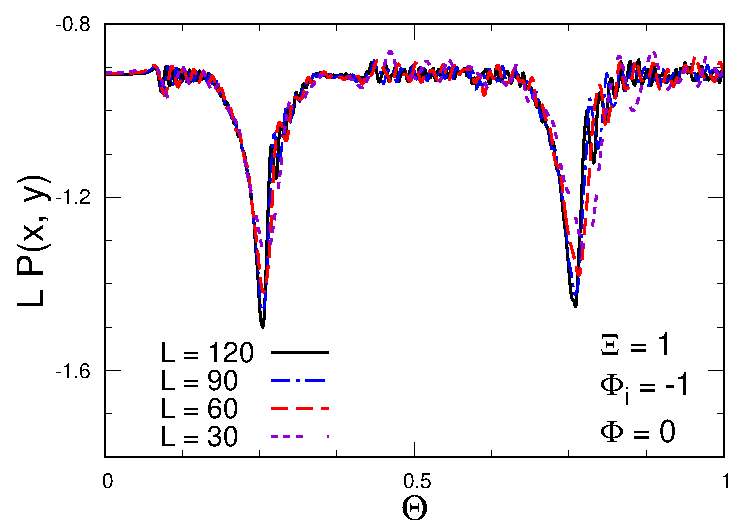
\includegraphics[width=0.6\columnwidth]{imm/LPk-1q0e100g0.pdf}
  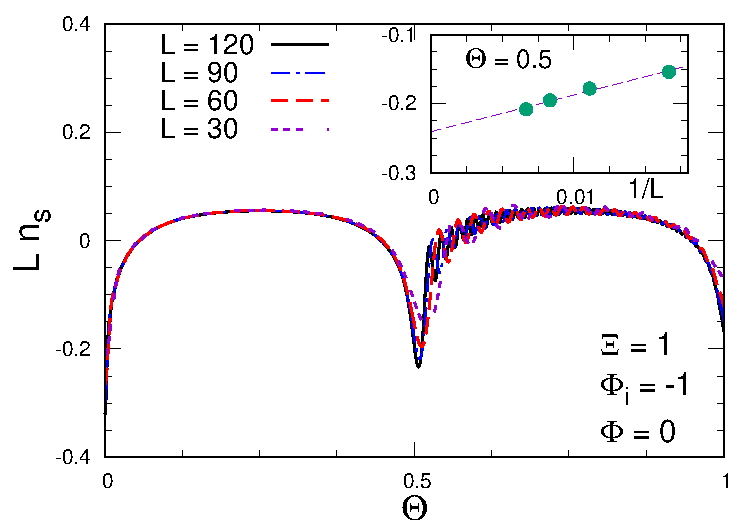
\includegraphics[width=0.6\columnwidth]{imm/LNk-1q0e100g0.pdf}
  \caption{OFSS behavior of the subtracted particle density (bottom)
    and the fermionic correlation function $P(x=L/3,y=2L/3,t)$,
    cf. Eq.~(\ref{ptf}), arising from the unitary QQ protocol, for
    various lattice sizes $L$, at fixed $\Xi=L^z T =1$,
    $\Phi_i=L^{y_w} w_i=-1$ and $\Phi=L^{y_w} w=0$, versus the time
    scaling variable $\Theta=t/L^z$.  These computations nicely
    support the OFSS behaviors reported in
    Eq.~(\ref{Oscaquefssa}). The inset of the bottom figure shows that
    the approach to the OFSS limit is consistent with $O(1/L)$
    corrections.  Analogous results are obtained for other values of
    the scaling variables.}
  \label{protares}
\end{figure}


The numerical analysis for the fermionic Kitaev wire under the unitary
protocol fully support to this OFSS, obtained by extending the QQ FSS
behaviors of closed systems starting from an initial ground
state. This is clearly demonstrated by the curves reported in
Fig.~\ref{protares}, associated with the quantum evolutions of the
subtracted particle density $n_s(t)$ and the fermionic correlation
$P(x,y,t)$ (the other fermionic correlation $C(x,y,t)$ develops an
analogous OFSS).



\subsubsection{OFSS along the dissipative QQ protocol}
\label{scalprotb}

We now discuss the dynamics arising from the dissipative protocol
outlined in Sec.~\ref{proto}, when the quantum evolution after
quenching is described by the Lindblad master equation
(\ref{Lindblad}) with the thermal-like dissipator (\ref{Dtrho}), to
modelize the interaction with a thermal bath characterized by a
temperature $T$ (which does not change after quenching)
and decay rate $\gamma$.

\begin{figure}[!htb]
\centering
  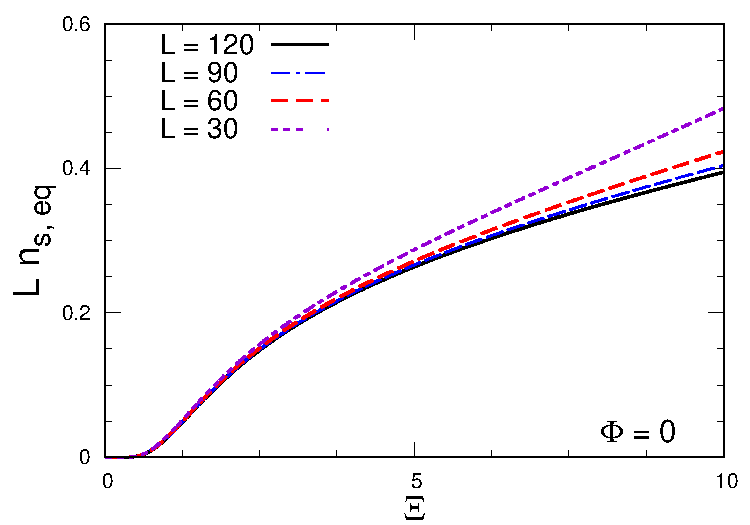
\includegraphics[width=0.6\columnwidth]{imm/LNeqXik0.pdf}
  \caption{ Equilibrium FSS of the subtracted particle density
    $n_{s,{\rm eq}}$ at the critical point $w=0$, versus the rescaled
    temperature $\Xi=L^z T$. With increasing $L$, the data show the
    expected convergence to the equilibrium FSS reported in
    Eq.~(\ref{nseqsca}) with $y_n=1$. }
  \label{eqns}
\end{figure}

  
\begin{figure}[!htb]
\centering
  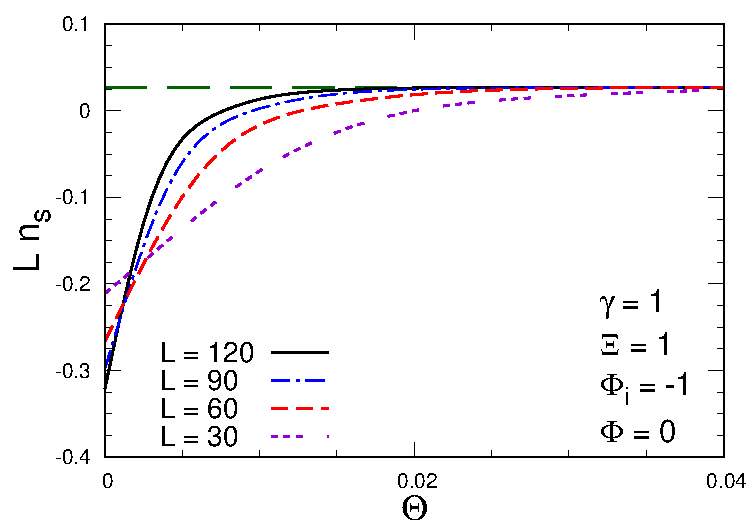
\includegraphics[width=0.6\columnwidth]{imm/LNk-1q0e100t100g1000.pdf}
  \caption{Quantum evolution of the subtracted particle density
    arising from the dissipative QQ protocol, when rescaling all
    quantities involved in the quench protocol, except for the decay
    rate $\gamma$. With increasing $L$, the curves appear to approach
    the equilibrium FSS value at finite temperature (where the
    temperature dependence enters through the scaling variable
    $\Xi=L^z T$) faster and faster, reflecting a nonuniform
    convergence for any $\Theta>0$. The dashed line shows the
    equilibrium value of $n_s$ for $\Phi=0$ and $\Xi=1$, which is
    asymptotically approached by the various curves.  }
  \label{protbresgamma}
\end{figure}



We expect that the temperature $T$ of the thermal bath must be
rescaled as in the case of the unitary QQ protocol, i.e. we must
consider again the associated scaling variable $\Xi$ already defined
in Eq.~(\ref{Xidef}).  However, since the QQ moves the system
out-of-equilibrium, also the decay rate $\gamma$, and corresponding
time scale $\tau=\gamma^{-1}$, associated with the interactions with
the thermal bath is expected to play a relevant role to establish a
corresponding nontrivial OFSS limit.  This was already noted in
Ref.~\cite{BD-23} in the analysis of dynamic protocols entailing the
variation of the temperature at the critical point.

When keeping $\tau$ constant in the FSS limit where the
scaling variable $\Theta=t/L^z$ is kept fixed, in the large-$L$ limit
we have eventually that
\begin{equation}
  t = \Theta \, L^z \gg \tau,
  \label{tggtau}
  \end{equation}
which is the condition ensuring thermalization for any finite value
$\Theta>0$. Therefore, when keeping $\tau$ fixed, the quantum
evolution is not expected to develop a nontrivial OFSS limit. Indeed,
in the large-$L$ limit, the system turns out to suddenly approach an
equilibrium Gibbs state (associated with the Hamiltonian parameter $w$
and temperature $T$) with respect to the rescaled time $\Theta$,
without any further relevant evolution of the system for any
$\Theta>0$.  Therefore, if the temperature is rescaled by keeping
$\Xi=L^z T$ fixed, we must recover the equilibrium FSS behavior in the
presence of a thermal bath at temperature $T$, such as that associated
with the subtracted particle density~\cite{CPV-14,RV-21}
\begin{equation}
  n_{s,{\rm eq}}(w,L,T) \approx L^{-y_n} {\cal N}(\Phi,\Xi),
  \label{nseqsca}
  \end{equation}
where $\Phi=L^{y_w} w$, and the temperature dependence enters through
the associated scaling variable $\Xi=L^z T$.  In Fig.~\ref{eqns} we
show some equilibrium data at the critical point $w=\Phi=0$, versus
$\Xi$, showing the approach to the asymptotic large-$L$ equilibrium
FSS (\ref{nseqsca}).  The realization of the equilibrium FSS within
the QQ protocol at fixed $\gamma$ is demonstrated by the plots
reported in Fig.~\ref{protbresgamma}, which show the somewhat trivial
convergence toward the equilibrium FSS for any finite $\Theta>0$.

The above results suggest that also the the decay rate $\gamma$ of the
system-bath interactions must be rescaled to observe a nontrivial OFSS
limit as a function of the time scaling variable $\Theta$, to create
the conditions for a balanced competition between the critical
Hamiltonian driving and the interactions with the thermal bath. As
already put forward in the case of other homogeneous dissipative terms
in the Lindblad equation~\cite{NRV-19-cd,RV-20-kz,TV-21,RV-21,FT-23},
for example associated with particle-decay or particle-pumping
dissipative mechanisms, a nontrivial OFSS limit is obtained by
rescaling the decay rate of the dissipative term, so that the scaling
variable
\begin{equation}
  \Gamma \equiv L^z \gamma \sim \gamma/\Delta
  \label{gammadef}
\end{equation}
is kept fixed in the OFSS limit, where $\Delta$ is the energy
difference of the lowest eigenstates of $\hat{H}(w)$ at the critical
point $w=w_c=0$.  Then an OFSS behavior emerges from the nontrivial
competition between the critical unitary dynamics and the dissipative
driving arising from the thermal bath.


\begin{figure}[!htb]
    \centering
      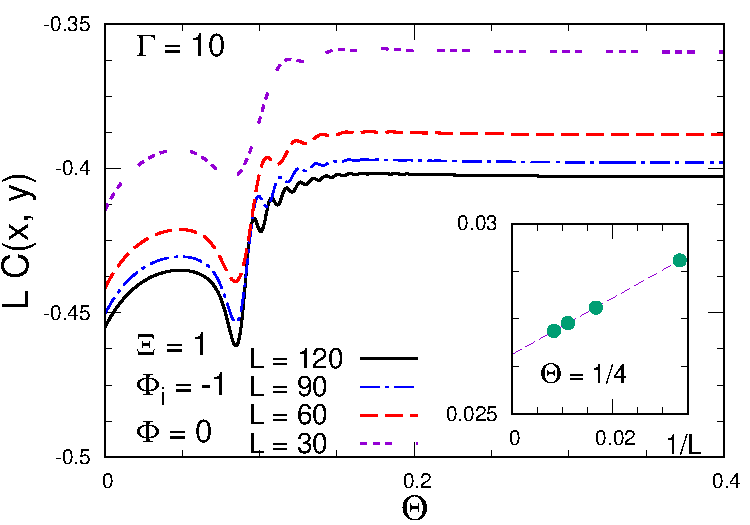
\includegraphics[width=0.45\columnwidth]{imm/LCk-1q0e100t100S10000.pdf}
      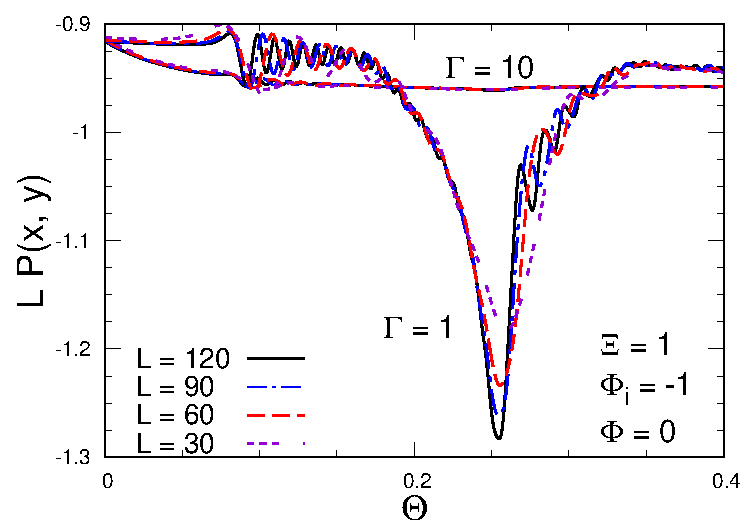
\includegraphics[width=0.45\columnwidth]{imm/LPk-1q0e100t100S10000.pdf}
        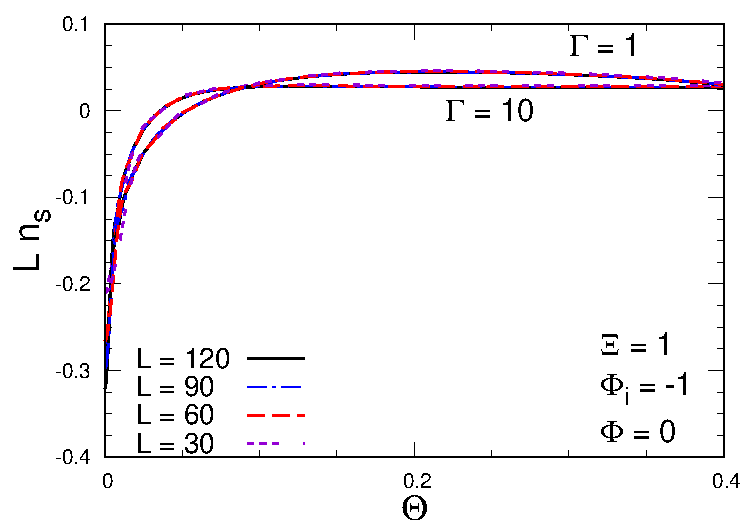
\includegraphics[width=0.45\columnwidth]{imm/LNk-1q0e100t100S10000.pdf}
        \caption{Quantum evolutions along the dissipative protocol, fully
          supporting the OFSS reported in Eqs.~(\ref{Oscaquefssprotb1})
          and (\ref{Oscaquefssprotb2}). We report curves for $L\,n_s$
          (bottom), $L\,P(x=L/3,y=2L/3,t)$ (middle), and
          $C(x=L/3,y=2L/3,t)$ (top), for various values of $L$, at fixed
          $\Phi_i=-1$, $\Phi=0$, $\Xi=1$, and two values of
          $\Gamma=L^z\gamma$, i.e.  $\Gamma=1,\,10$ (except for the top
          figure where we only report data for $\Gamma=10$ to ensure a
          good readability).  The inset of the top figure shows that the
          OFSS is approached with $O(1/L)$ corrections. Analogous results
          are obtained for other values of the scaling variables. }
      \label{protbresgammaresc}
\end{figure}

In conclusion, on the basis of the above scaling arguments, the OFSS
arising from the dissipative QQ protocols in the presence of a thermal
bath is expected to be given by
\begin{eqnarray}
   O_a(t, L, w_i, w, T, \gamma) \, \approx \, L^{-y_o} \,
  {\cal O}_a(\Theta, \Phi_i, \Phi, \Xi, \Gamma),\quad
  \label{Oscaquefssprotb1}
\end{eqnarray}
and
\begin{eqnarray}
&& G_{O}(t, {\bm x}_1, {\bm x}_2, L, w_i, w, T, \gamma)  \, \approx
    \label{Oscaquefssprotb2} \\
    &&\qquad\qquad
     L^{-2y_o} \, {\cal G}_{O}(\Theta, {\bm X}_1, {\bm X}_2, \Phi_i,
    \Phi, \Xi, \Gamma). \qquad \nonumber
\end{eqnarray}
In the large-$\Gamma$ limit the above OFFS behaviors at fixed $\Xi$ is
expected to approach the corresponding equilibrium FSS, faster and
faster in terms of $\Theta$, matching the behavior at finite $\gamma$.
Moreover, we also expect that the equilibrium FSS is also approached
in the large-$\Theta$ limit at fixed $\Gamma$ and $\Xi$, independently
of $\Gamma$, but faster and faster with increasing~$\Gamma$.

Again, the numerical results for the particle density $n_s(t)$ and
correlation functions $P$ and $C$ fully support the above OFSS
equations, i.e. Eq.~(\ref{Oscaquefssprotb1}) for $n_s(t)$ with
$y_o=y_n=1$, and Eq.~(\ref{Oscaquefssprotb2}) for $P$ and $C$ with
$y_o=y_c=1/2$. Some results are reported in
Fig.~\ref{protbresgammaresc}.  We also stress that analogous results
are expected for other observables, for example the correlation
functions of the spin operator of the equivalent formulation provided
by the quantum Ising chains.


